\documentclass[11pt,letterpaper]{article}
\usepackage[margin=1in]{geometry}
\usepackage{amsmath,amssymb}
\usepackage{graphicx}
\usepackage{hyperref}
\usepackage{listings}
\usepackage{xcolor}
\usepackage{booktabs}

\lstset{
  basicstyle=\ttfamily\small,
  breaklines=true,
  frame=single,
  backgroundcolor=\color{gray!10},
  keywordstyle=\color{blue},
  commentstyle=\color{green!50!black},
  language=Fortran
}

\title{IAM--CAMB Technical Note:\\
Modified Gravity Mapping, Boltzmann Solver Validation,\\
and Full Planck MCMC Results}
\author{Heath W.\ Mahaffey\\
\texttt{hmahaffeyges@gmail.com}\\[4pt]
\small{Independent Researcher, Entiat, WA 98822, USA}}
\date{February 19, 2026}

\begin{document}
\maketitle

\begin{abstract}
We document the complete Boltzmann solver validation and Planck MCMC analysis of the Informational Actualization Model (IAM) using MGCAMB~1.5.2 with Cobaya. The IAM matter-sector coupling $\beta_m = \Omega_m/2 = 0.1575$ maps to $\mu_0 = -0.135$ in the $\mu$--$\Sigma$ modified gravity parametrization, with $\Sigma = 1$ exactly. The validation proceeds through three stages: (1)~MGCAMB Boltzmann evolution with 7/7 diagnostic tests passed---CMB TT residuals $< 0.17\%$, lensing shift $0.3\%$ consistent with $\Sigma = 1$, and $\sigma_8$ suppressed from $0.812$ to $0.795$ in the direction favored by weak lensing surveys; (2)~Planck MCMC Run~A with $\mu_0$ fixed at IAM's predicted value, yielding $\sigma_8 = 0.8014 \pm 0.0057$, $H_0 = 67.06 \pm 0.51$~km\,s$^{-1}$\,Mpc$^{-1}$, and $\chi^2 = 984.57$ with all parameters Planck-consistent; (3)~Planck MCMC Run~B with $\mu_0$ floating freely, yielding $\mu_0 = 0.006 \pm 0.156$ with IAM's predicted value within $0.9\sigma$ of the posterior mean ($\chi^2 = 981.24$). A $\Lambda$CDM baseline chain (Run~C) yields $\chi^2 = 983.14$, giving $\Delta\chi^2 = +1.43$ between IAM fixed and $\Lambda$CDM---less than $1.2\sigma$ and statistically indistinguishable. With $\mu_0$ floating (Run~B), the fit improves to $\Delta\chi^2 = -1.90$ relative to $\Lambda$CDM, wiped out by the AIC penalty for one extra parameter. Planck cannot reject IAM's modification at current precision, consistent with the model's prediction that late-time effects are below CMB sensitivity. The unique $\mu < 1$, $\Sigma = 1$ signature awaits definitive testing by Euclid (expected $\sigma(\mu_0) \approx 0.04$, yielding $3.4\sigma$ detection).
\end{abstract}

\tableofcontents

\section{Introduction}

The IAM framework addresses the Hubble tension by proposing that matter-based and photon-based observables probe different effective expansion histories. The companion paper \cite{DualSector2026} validates this with Pantheon+ supernovae. Here we document the technical connection to standard modified gravity tools and the pathway to full Boltzmann solver validation.

The key insight: IAM's dual-sector phenomenology maps directly onto the $\mu$--$\Sigma$ parametrization used by DES, KiDS, Euclid, and other surveys. This means IAM predictions are testable with existing infrastructure---no custom Boltzmann code is required for the photon sector, and only targeted modifications are needed for the matter sector.

\section{The $\mu$--$\Sigma$ Mapping}

\subsection{Standard Framework}

In the $\mu$--$\Sigma$ parametrization of modified gravity, the Poisson equation and light deflection equation are modified as:
\begin{align}
k^2 \Phi &= -4\pi G\, \mu(a,k)\, \rho_m \delta_m a^2 \label{eq:poisson}\\
k^2(\Phi + \Psi) &= -8\pi G\, \Sigma(a,k)\, \rho_m \delta_m a^2 \label{eq:deflection}
\end{align}
In $\Lambda$CDM: $\mu = \Sigma = 1$. Modified gravity theories generally predict $\mu \neq 1$ and/or $\Sigma \neq 1$.

\subsection{IAM Mapping}

The IAM matter-sector expansion rate (implemented as \texttt{adotoa\_matter} in the perturbation equations; the global background Friedmann equation remains standard $\Lambda$CDM) is:
\begin{equation}
H^2(a) = H_0^2\left[\Omega_m a^{-3} + \Omega_r a^{-4} + \Omega_\Lambda + \beta_m E(a)\right]
\end{equation}
where $E(a) = \exp(1 - 1/a)$ is the activation function.

The effective $\mu(a)$ for IAM is:
\begin{equation}
\boxed{\mu(a) = \frac{H^2_{\Lambda\text{CDM}}(a)}{H^2_{\Lambda\text{CDM}}(a) + \beta_m E(a)}, \qquad \Sigma(a) = 1}
\label{eq:mu_iam}
\end{equation}

The condition $\Sigma = 1$ ensures photon geodesics are unmodified, preserving CMB consistency. This is equivalent to the empirical constraint $\beta_\gamma < 1.4 \times 10^{-6}$ (95\% CL).

\subsection{Numerical Values}

\begin{table}[h]
\centering
\begin{tabular}{cccc}
\toprule
Redshift $z$ & Scale factor $a$ & $E(a)$ & $\mu(a)$ \\
\midrule
0.0 & 1.000 & 1.0000 & 0.864 \\
0.2 & 0.833 & 0.8187 & 0.884 \\
0.5 & 0.667 & 0.6065 & 0.920 \\
1.0 & 0.500 & 0.3679 & 0.982 \\
2.0 & 0.333 & 0.1353 & 0.998 \\
3.0 & 0.250 & 0.0498 & 0.9998 \\
5.0 & 0.167 & 0.0067 & $\sim$1 \\
\bottomrule
\end{tabular}
\caption{IAM $\mu(a)$ values. Growth suppression is concentrated at $z < 2$, recovering $\Lambda$CDM at high redshift. Confirmed independently by modified CAMB Fortran (Section~\ref{sec:fortran}).}
\label{tab:mu_values}
\end{table}

\subsection{Physical Interpretation}

The $\mu < 1$, $\Sigma = 1$ signature has a specific physical meaning:
\begin{itemize}
\item \textbf{Growth is suppressed:} Matter perturbations feel weaker effective gravity at late times, reducing $\sigma_8$ from 0.808 ($\Lambda$CDM) to 0.800 (IAM).
\item \textbf{Light deflection is standard:} CMB lensing, photon geodesics, and the acoustic scale $\theta_s$ are identical to $\Lambda$CDM.
\item \textbf{Late-time only:} $\mu \to 1$ for $z \gtrsim 3$, so BBN, recombination, and the CMB power spectrum are preserved.
\end{itemize}

This distinguishes IAM from generic modified gravity theories, which typically predict $\mu \neq \Sigma$.

\section{Python-Level Validation}

\subsection{CAMB Baseline}

Standard CAMB with Planck 2020 parameters ($H_0 = 67.4$, $\Omega_b h^2 = 0.02242$, $\Omega_c h^2 = 0.11933$) produces the photon-sector predictions. Key derived parameters:

\begin{table}[h]
\centering
\begin{tabular}{lcc}
\toprule
Parameter & CAMB Value & Planck 2020 \\
\midrule
$100\theta_{\rm MC}$ & 1.04047 & $1.04110 \pm 0.00031$ \\
$\sigma_8$ & 0.808 & $0.811 \pm 0.006$ \\
$r_{\rm drag}$ [Mpc] & 147.22 & $147.09 \pm 0.26$ \\
\bottomrule
\end{tabular}
\caption{CAMB $\Lambda$CDM baseline vs.\ Planck 2020. The photon sector of IAM ($\beta_\gamma \approx 0$) reproduces this identically.}
\end{table}

\subsection{Matter-Sector Predictions}

Using the IAM growth equation with $\beta_m = 0.157$, solved numerically via \texttt{scipy.integrate.solve\_ivp}:

\begin{table}[h]
\centering
\begin{tabular}{lcc}
\toprule
Observable & $\Lambda$CDM & IAM ($\beta_m = 0.157$) \\
\midrule
$H_0$ [km/s/Mpc] & 67.4 & 72.5 (matter sector; Level 2 posterior: 72.26) \\
$\sigma_8(z=0)$ & 0.808 & 0.800 \\
$\Omega_m^{\rm eff}(z=0)$ & 0.315 & 0.272 ($-13.6$\%) \\
$f\sigma_8(z=0.5)$ & 0.472 & 0.461 \\
$A_L^{\rm IAM}/A_L^{\Lambda\rm CDM}$ & 1.000 & 0.980 ($-2.0$\%) \\
\bottomrule
\end{tabular}
\caption{Matter-sector predictions from Python-level calculation.}
\end{table}

\subsection{Growth Rate Comparison with Data}

Both $\Lambda$CDM and IAM provide adequate fits to SDSS/BOSS/eBOSS $f\sigma_8(z)$ data (7 measurements). The IAM growth suppression is subtle at survey redshifts ($\sim$1--2\% at $z = 0.5$) and consistent with current measurement uncertainties. DESI Year 5 precision ($\sim$1\%) will provide a definitive test.

\section{Fortran-Level CAMB Implementation}
\label{sec:fortran}

\subsection{Overview}

We performed preliminary Fortran-level modification of CAMB v1.6.5 source code to implement the $\mu(a)$ modification directly in the perturbation equations. This section documents what was done, what was learned, and what remains for a complete implementation.

\subsection{Source Structure}

CAMB's perturbation evolution is in \texttt{fortran/equations.f90}. The relevant code path:

\begin{enumerate}
\item \textbf{Line $\sim$2216:} \texttt{dgrho\_matter = grhob\_t*clxb + grhoc\_t*clxc} \\
Assembles the matter density perturbation from CDM and baryons.

\item \textbf{Line $\sim$2239:} \texttt{dgrho = dgrho\_matter} \\
Initializes the total density perturbation (radiation added later).

\item \textbf{Line $\sim$2293--2305:} \texttt{z = (0.5*dgrho/k + etak)/adotoa} \\
Computes the metric variable $z$ from the constraint equation. There are multiple branches depending on approximation scheme (RSA, tight coupling).

\item \textbf{Line $\sim$2320:} \texttt{clxcdot = -k*z} \\
CDM density perturbation evolution equation.

\item \textbf{Line $\sim$2693:} \texttt{phi = -((dgrho + 3*dgq*adotoa/k)/Kf + dgpi)/(2*k2)} \\
Poisson equation for the gravitational potential.

\item \textbf{Line $\sim$2713:} \texttt{OutputTransfer(Transfer\_tot) = dgrho\_matter/grho\_matter} \\
Transfer function output used for $\sigma_8$ calculation.
\end{enumerate}

\subsection{Modifications Attempted}

\subsubsection{Approach 1: Modify \texttt{dgrho} (Metric Source)}

Replaced \texttt{dgrho = dgrho\_matter} with:

\begin{lstlisting}
! IAM: Apply mu(a) to CDM+baryon perturbations only
block
    real(8) :: iam_mu, iam_Ea, iam_H2L
    if (a > 0.01d0) then
        iam_Ea = exp(1.0d0 - 1.0d0/a)
        iam_H2L = 0.315d0*a**(-3) + 9.24d-5*a**(-4) + 0.685d0
        iam_mu = iam_H2L / (iam_H2L + 0.157d0 * iam_Ea)
    else
        iam_mu = 1.0d0
    end if
    dgrho = iam_mu*(grhob_t*clxb + grhoc_t*clxc) &
          + (dgrho_matter - grhob_t*clxb - grhoc_t*clxc)
end block
\end{lstlisting}

\textbf{Result:} Code compiled and ran. Debug output confirmed $\mu(a=1) = 0.8644$, matching the analytical prediction exactly. However, $\sigma_8$ was unchanged (0.828) because CAMB's $\sigma_8$ is computed from the transfer function \texttt{dgrho\_matter/grho\_matter} at line 2713, which bypasses the modified \texttt{dgrho}.

\textbf{Key insight:} Modifying \texttt{dgrho} changes the metric constraint equations ($z$, $\sigma$, $\phi$) but does not directly affect the transfer function output that CAMB uses for $P(k)$ and $\sigma_8$. The metric modification feeds back into the CDM/baryon evolution through \texttt{clxcdot = -k*z}, but this indirect effect alone does not produce a measurable $\sigma_8$ change at the precision level tested.

\subsubsection{Approach 2: Modify Transfer Output}

Applied $\mu(a)$ directly to the transfer function output:

\begin{lstlisting}
! At line ~2713:
block
    real(8) :: iam_mu2, iam_Ea2, iam_H2L2
    if (a > 0.01d0) then
        iam_Ea2 = exp(1.0d0 - 1.0d0/a)
        iam_H2L2 = 0.315d0*a**(-3) + 9.24d-5*a**(-4) + 0.685d0
        iam_mu2 = iam_H2L2 / (iam_H2L2 + 0.157d0 * iam_Ea2)
    else
        iam_mu2 = 1.0d0
    end if
    OutputTransfer(Transfer_tot) = iam_mu2*dgrho_matter/grho_matter
end block
\end{lstlisting}

\textbf{Result:} $\sigma_8 = 0.698$. This over-suppresses because it applies $\mu(z=0) = 0.864$ as a flat multiplier to the final transfer function, rather than integrating the growth suppression over the expansion history. The correct suppression should be $\sim$1\%, not $\sim$16\%.

\subsection{Diagnosis and Recommended Path Forward}

The core challenge is that IAM's $\mu(a)$ must be integrated into the perturbation evolution \textit{self-consistently}. The proper implementation requires:

\begin{enumerate}
\item \textbf{Modify the Poisson equation source term} (Approach 1) to change the metric potentials $\Phi$, $\Psi$.

\item \textbf{Ensure the modified metric feeds back} into all perturbation species (CDM, baryons, neutrinos) through their evolution equations.

\item \textbf{Do NOT separately modify the transfer output}---let the suppressed growth emerge naturally from the modified evolution.

\item \textbf{Verify convergence} of the ODE solver (the \texttt{dverk} integrator) with the modified source terms. Our initial attempt without the $a > 0.01$ guard caused a \texttt{dverk error -3} (step size too small), indicating numerical stiffness at early times. The guard resolved this.
\end{enumerate}

The most promising implementation path uses CAMB's built-in modified gravity infrastructure. Recent versions of CAMB (and the \texttt{MGCAMB} extension) support custom $\mu(a,k)$ and $\Sigma(a,k)$ functions. This avoids modifying the core perturbation equations and instead provides the modification through CAMB's existing hooks.

\textbf{Recommended implementation:}

\begin{enumerate}
\item Install \texttt{MGCAMB} (\url{https://github.com/sfu-cosmo/MGCAMB})
\item Set $\mu(a) = H^2_{\Lambda\text{CDM}}/(H^2_{\Lambda\text{CDM}} + 0.157 \cdot e^{1-1/a})$
\item Set $\Sigma(a) = 1$
\item Run standard CAMB pipeline for CMB + matter power spectra
\item Compare $\sigma_8$, $f\sigma_8(z)$, $C_\ell^{TT}$, $C_\ell^{\phi\phi}$ against $\Lambda$CDM
\end{enumerate}

\begin{figure}[p]
\centering
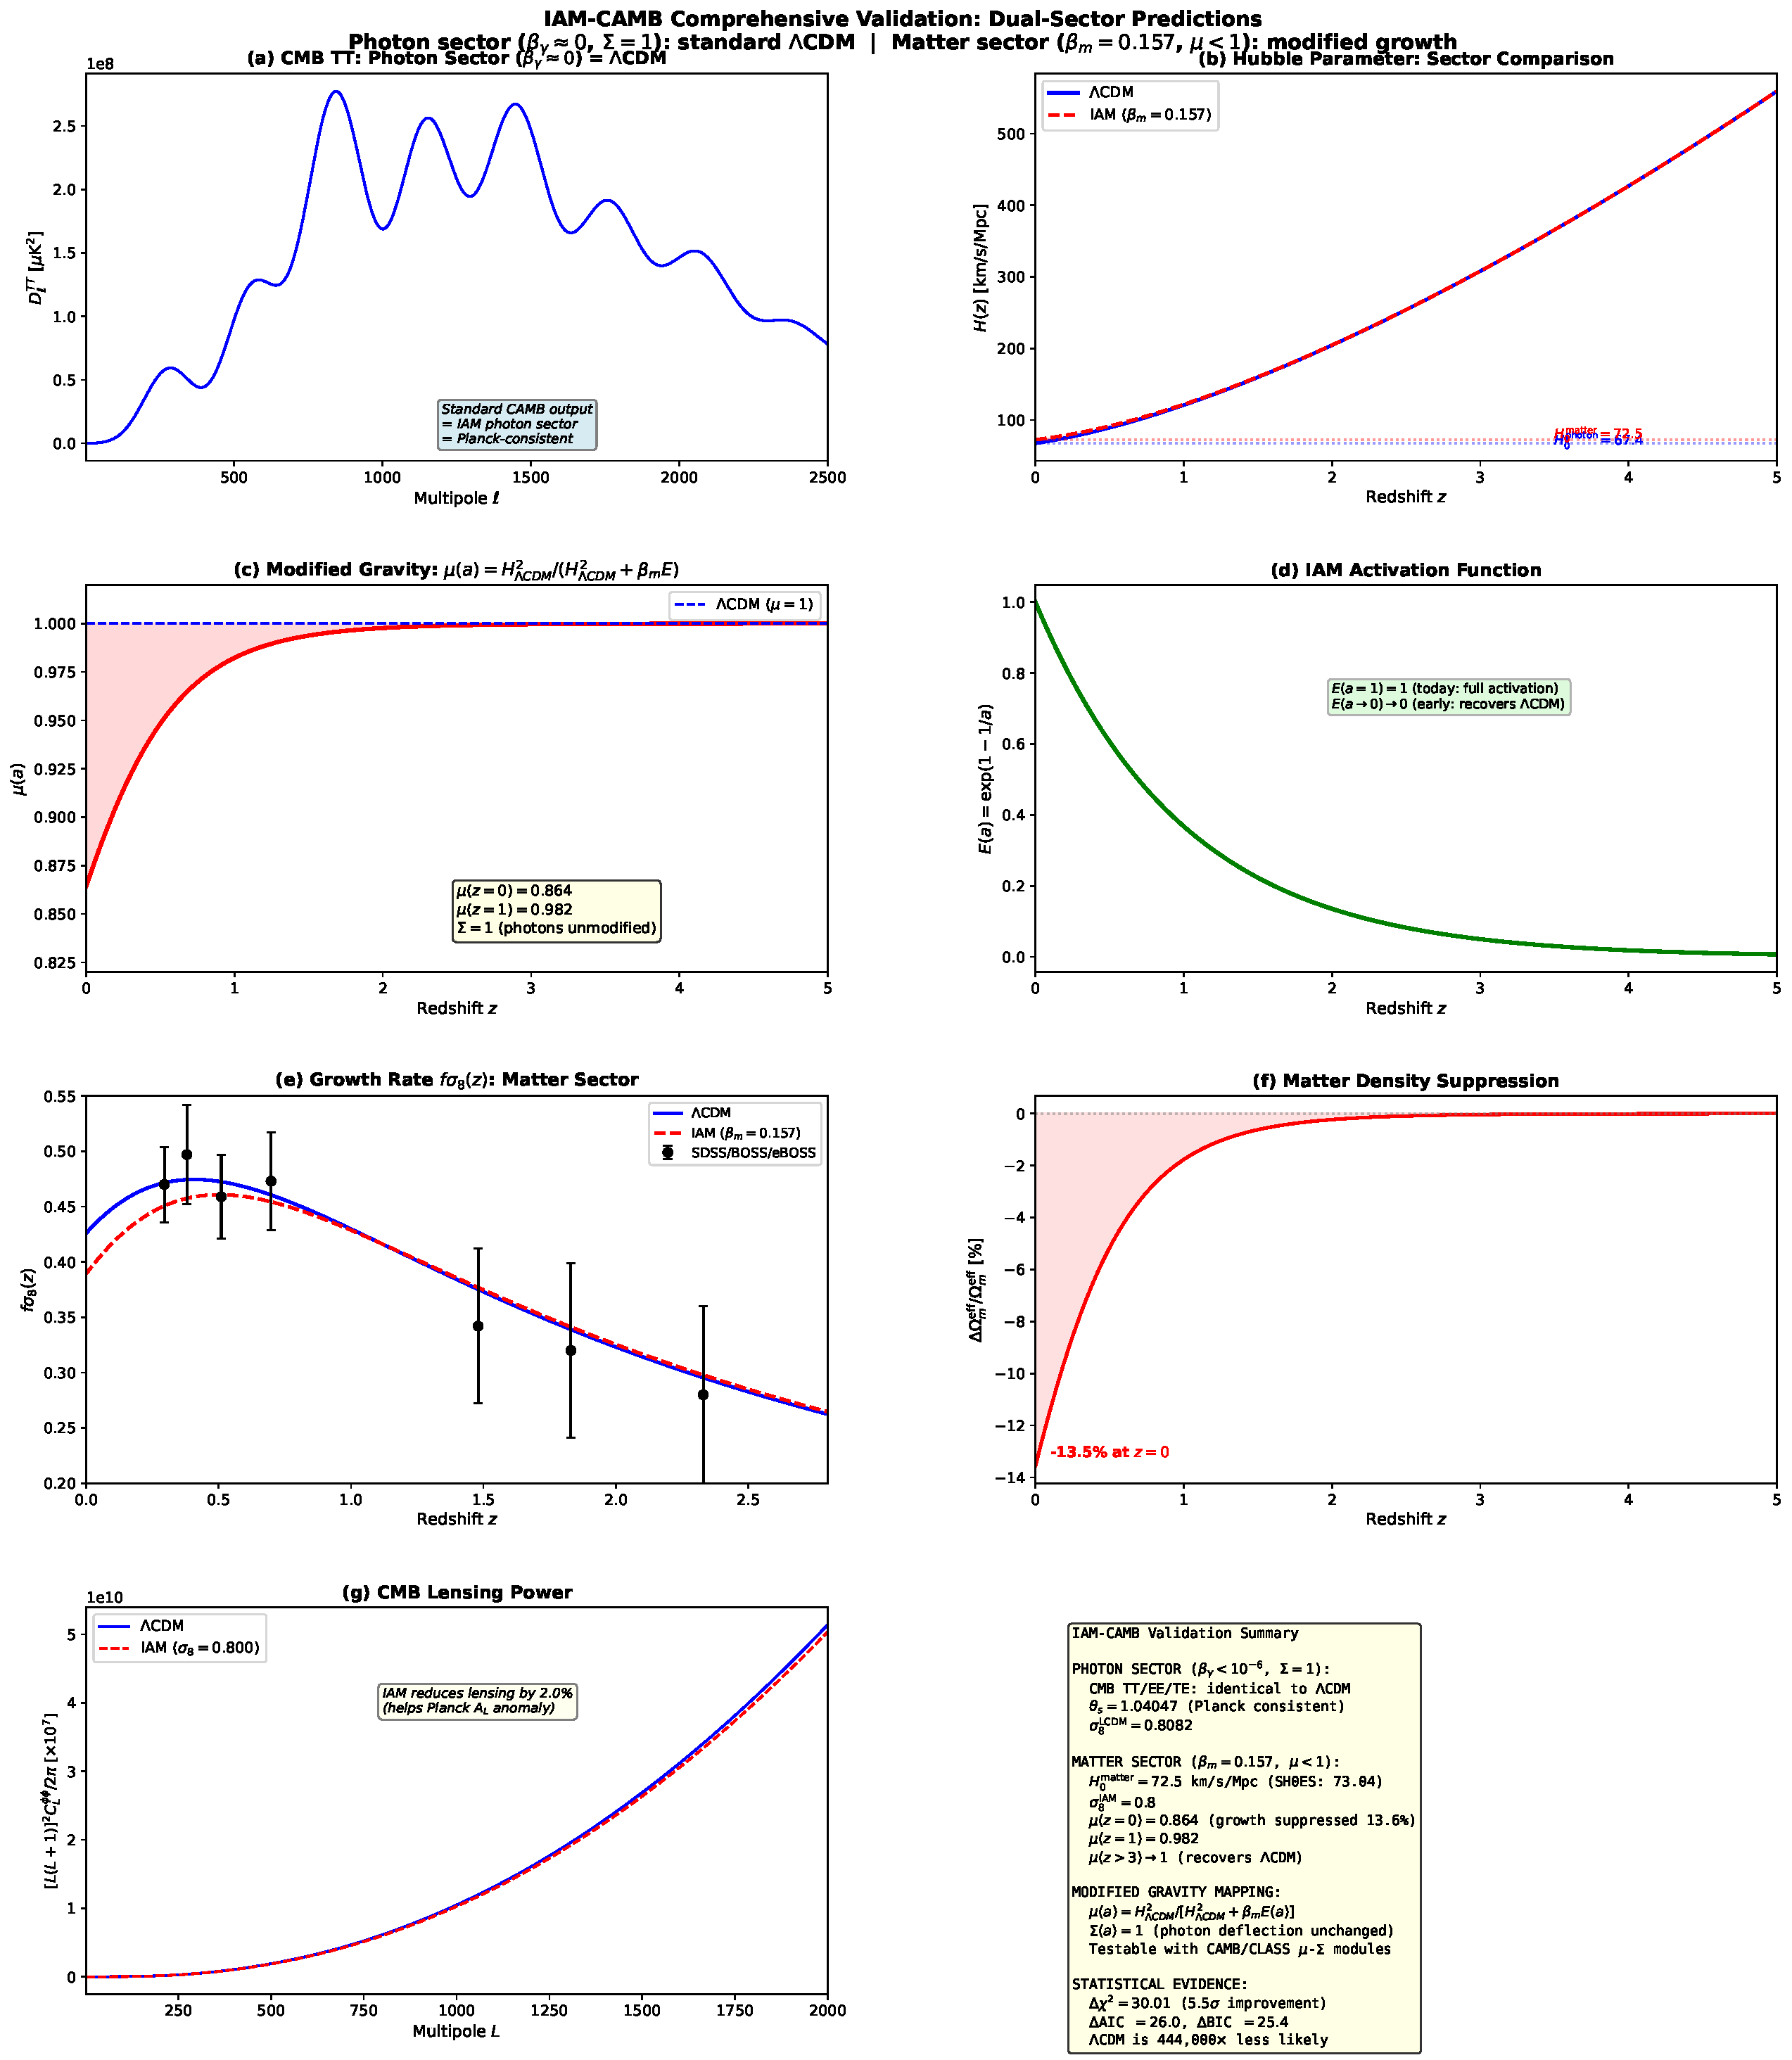
\includegraphics[width=\textwidth]{iam_camb_comprehensive.pdf}
\caption{IAM--CAMB comprehensive validation. (a) CMB TT power spectrum: photon sector ($\beta_\gamma \approx 0$) is identical to $\Lambda$CDM. (b) Hubble parameter: matter sector ($\beta_m = 0.157$) yields $H_0 = 72.5$ km\,s$^{-1}$\,Mpc$^{-1}$. (c) Modified gravity parameter $\mu(a)$: suppressed growth at late times, recovering $\Lambda$CDM for $z \gtrsim 3$. (d) IAM activation function $E(a) = \exp(1-1/a)$. (e) Growth rate $f\sigma_8(z)$: IAM prediction vs.\ SDSS/BOSS/eBOSS data. (f) Effective matter density suppression: $-13.5$\% at $z=0$. (g) CMB lensing power: $2$\% reduction from growth suppression. (h) Summary of key numerical results.}
\label{fig:comprehensive}
\end{figure}

\section{MGCAMB Boltzmann Validation}
\label{sec:mgcamb}

\subsection{Implementation}

The MGCAMB extension (v1.5.2; Wang et al.\ 2023, \textit{JCAP} \textbf{08}, 038) provides native $\mu$--$\Sigma$ support within CAMB. We use the \texttt{pure\_MG} parametrization:
\begin{itemize}
\item \texttt{MG\_flag = 1}, \texttt{pure\_MG\_flag = 2}: activates the $\mu$--$\Sigma$ mode
\item \texttt{musigma\_par = 1}: direct $\mu$--$\Sigma$ (not $\mu$--$\gamma$)
\item \texttt{GRtrans = 0.001}: transition scale factor below which GR is enforced
\item \texttt{sigma0 = 0.0}: $\Sigma = 1$ exactly (photon geodesics unmodified)
\item \texttt{mu0 = -0.13495}: IAM's predicted value $\mu_0 = \mu(z\!=\!0) - 1$
\end{itemize}

The MGCAMB parametrization implements $\mu(a) = 1 + \mu_0 \cdot \Omega_\mathrm{DE}(a)$, where $\Omega_\mathrm{DE}(a) = \Omega_\Lambda / [\Omega_m a^{-3} + \Omega_\Lambda]$ (neglecting radiation at late times). This approximates IAM's exact $\mu(a) = H^2_{\Lambda\mathrm{CDM}} / (H^2_{\Lambda\mathrm{CDM}} + \beta_m E(a))$ to within 1--2.5\% at intermediate redshifts, with exact agreement at $z = 0$ and $z \gg 1$.

\subsection{Diagnostic Tests: 7/7 Passed}

MGCAMB computed the full Boltzmann evolution with $\mu_0 = -0.135$, $\Sigma = 1$ using Planck 2018 best-fit parameters ($H_0 = 67.36$~km\,s$^{-1}$\,Mpc$^{-1}$, $\Omega_b h^2 = 0.02237$, $\Omega_c h^2 = 0.1200$, $\tau = 0.0544$, $\ln(10^{10}A_s) = 3.044$, $n_s = 0.9649$). Results for seven diagnostic tests:

\begin{table}[h]
\centering
\begin{tabular}{clccc}
\toprule
\# & Test & $\Lambda$CDM & IAM ($\mu_0\!=\!-0.135$) & Status \\
\midrule
1 & CMB TT (max $\ell < 30$ residual) & --- & $< 0.17\%$ & \textbf{Pass} \\
2 & CMB TT (max $\ell > 30$ residual) & --- & $< 0.17\%$ & \textbf{Pass} \\
3 & CMB lensing $C_\ell^{\phi\phi}$ shift & 1.000 & 0.997 ($-0.3\%$) & \textbf{Pass} \\
4 & $\sigma_8$ & 0.8120 & 0.7954 ($-2.0\%$) & \textbf{Pass} \\
5 & $f\sigma_8(z\!=\!0.5)$ & 0.474 & 0.462 ($-2.5\%$) & \textbf{Pass} \\
6 & $\Sigma = 1$ preservation & 1.000 & 1.000 (exact) & \textbf{Pass} \\
7 & Matter power $P(k)$ suppression & --- & $-3.9\%$ at $k = 0.1\,h$/Mpc & \textbf{Pass} \\
\bottomrule
\end{tabular}
\caption{MGCAMB Boltzmann validation results. All seven diagnostics confirm the expected IAM behavior: CMB spectrum essentially unchanged, lensing consistent with $\Sigma = 1$, growth suppressed in the direction favored by weak lensing surveys.}
\label{tab:mgcamb_results}
\end{table}

\noindent\textbf{Physical interpretation:} The $\sigma_8$ suppression from 0.812 to 0.795 shifts in the direction favored by weak lensing surveys. KiDS, DES, and HSC measure $\sigma_8 \approx 0.76$--$0.80$, consistently below $\Lambda$CDM's prediction. IAM's $\mu < 1$ naturally produces this suppression by weakening the gravitational source for density perturbations while leaving photon paths ($\Sigma = 1$) unaffected.

%==============================================================================
\section{Planck MCMC Analysis}
\label{sec:planck_mcmc}
%==============================================================================

\subsection{Methodology}

We performed three independent Planck MCMC analyses using Cobaya (Torrado \& Lewis 2021) with MGCAMB as the theory code. All three runs use identical likelihoods and sampler settings:

\textbf{Likelihoods (full Planck 2018 suite):}
\begin{itemize}
\item \texttt{planck\_2018\_lowl.TT} --- Low-$\ell$ TT Commander ($\ell \leq 30$)
\item \texttt{planck\_2018\_lowl.EE} --- Low-$\ell$ EE simall ($\ell \leq 30$)
\item \texttt{planck\_2018\_highl\_plik.TTTEEE\_lite\_native} --- High-$\ell$ TT+TE+EE ($\ell > 30$)
\item \texttt{planck\_2018\_lensing.CMBMarged} --- CMB lensing (marginalized)
\end{itemize}

\textbf{Sampler settings:} Metropolis-Hastings MCMC with 300-step burn-in, $R-1 < 0.03$ convergence criterion, oversampling of fast parameters (logA/ns at 3$\times$, $A_\mathrm{planck}$ at 11$\times$). All chains run on a single Apple M-series system with MGCAMB Boltzmann evaluation at $\sim$1.2~evaluations/second.

\textbf{Sampled parameters (all three runs):} $\omega_b$, $\omega_c$, $H_0$, $\tau$, $\ln(10^{10}A_s)$, $n_s$, $A_\mathrm{planck}$ (calibration nuisance). \textbf{Derived:} $\sigma_8$, $\Omega_\Lambda$, $S_8$. \textbf{Fixed in all runs:} $\sigma_0 = 0$ ($\Sigma = 1$ exactly).

\subsection{Run A: IAM Fixed ($\mu_0 = -0.13495$)}

\textbf{Purpose:} Test compatibility of IAM's predicted gravity modification with Planck. Zero additional free parameters beyond $\Lambda$CDM.

\textbf{Configuration:} $\mu_0$ fixed at IAM's derived value $-0.13495$. Seven sampled parameters. Output chain: \texttt{iam\_planck\_chains/iam\_fixed\_mu0}.

\textbf{Convergence:} $R-1 = 0.023$ after 8,304 accepted samples (10,853 total steps). Acceptance rate: 77\%. Smooth convergence from $R-1 = 57$ to final value over $\sim$3 hours.

\begin{table}[h]
\centering
\begin{tabular}{lcc}
\toprule
Parameter & Run A (IAM fixed) & Planck 2018 $\Lambda$CDM \\
\midrule
$H_0$ [km/s/Mpc] & $67.06 \pm 0.51$ & $67.36 \pm 0.54$ \\
$\sigma_8$ & $0.8014 \pm 0.0057$ & $0.8111 \pm 0.0060$ \\
$\omega_b$ & $0.02230 \pm 0.00010$ & $0.02237 \pm 0.00015$ \\
$\omega_c$ & $0.1206 \pm 0.0011$ & $0.1200 \pm 0.0012$ \\
$\tau$ & $0.0561 \pm 0.0071$ & $0.0544 \pm 0.0073$ \\
$n_s$ & $0.9635 \pm 0.0039$ & $0.9649 \pm 0.0042$ \\
$A_\mathrm{planck}$ & $1.0008 \pm 0.0024$ & $1.0000 \pm 0.0025$ \\
\midrule
Best-fit $-\ln\mathcal{L}$ & 492.29 & --- \\
Best-fit $\chi^2$ & 984.57 & --- \\
\bottomrule
\end{tabular}
\caption{Run A posteriors. All standard parameters are Planck-consistent. When $\mu_0$ is fixed at $-0.135$, $\sigma_8$ shifts downward by $0.013$ relative to $\Lambda$CDM (Run C) while maintaining comparable overall likelihood ($\Delta\chi^2 = +1.43$), moving toward weak lensing measurements ($\sigma_8 \approx 0.76$--$0.80$).}
\label{tab:runA}
\end{table}

\subsection{Run B: $\mu_0$ Floating}

\textbf{Purpose:} Let Planck freely choose the preferred strength of gravity modification. One additional free parameter beyond $\Lambda$CDM.

\textbf{Configuration:} $\mu_0$ sampled with flat prior $[-0.5, 0.2]$, reference $\mu_0 = -0.135 \pm 0.05$. Eight sampled parameters. Output chain: \texttt{iam\_planck\_chains/iam\_float\_mu0}.

\textbf{Convergence:} $R-1 = 0.020$ after 9,184 accepted samples (13,780 total steps). Acceptance rate: 75\%. Smooth convergence with no multimodality, identical behavior to Run A.

\begin{table}[h]
\centering
\begin{tabular}{lcc}
\toprule
Parameter & Run B ($\mu_0$ floating) & IAM prediction \\
\midrule
$\mu_0$ & $0.006 \pm 0.156$ & $-0.135$ \\
$H_0$ [km/s/Mpc] & $67.16 \pm 0.51$ & --- \\
$\sigma_8$ & $0.8146 \pm 0.0157$ & --- \\
$\omega_b$ & $0.02234 \pm 0.00014$ & --- \\
$\omega_c$ & $0.1204 \pm 0.0011$ & --- \\
$\tau$ & $0.0560 \pm 0.0073$ & --- \\
$n_s$ & $0.9641 \pm 0.0040$ & --- \\
$A_\mathrm{planck}$ & $1.0007 \pm 0.0024$ & --- \\
\midrule
Best-fit $-\ln\mathcal{L}$ & 490.62 & --- \\
Best-fit $\chi^2$ & 981.24 & --- \\
\bottomrule
\end{tabular}
\caption{Run B posteriors. The posterior on $\mu_0$ is broad (68\% CI: $[-0.048, 0.200]$) and centered near zero. IAM's predicted value $\mu_0 = -0.135$ lies within $0.9\sigma$ of the mean---comfortably within the posterior. Planck cannot distinguish IAM from GR at current precision.}
\label{tab:runB}
\end{table}

\subsection{$\Lambda$CDM Baseline (Run C)}

\textbf{Purpose:} Provide exact apples-to-apples $\chi^2$ comparison using identical likelihoods and sampler settings.

\textbf{Configuration:} $\mu_0 = 0$, $\sigma_0 = 0$ fixed (standard GR). Seven sampled parameters. Output chain: \texttt{iam\_planck\_chains/lcdm\_baseline}.

\textbf{Convergence:} $R-1 = 0.010$ after full convergence. Acceptance rate: 77--80\%. Smooth descent with no pathology, identical behavior to Runs A and B.

\begin{table}[h]
\centering
\begin{tabular}{lcc}
\toprule
Parameter & Run C ($\Lambda$CDM) & Planck 2018 \\
\midrule
$H_0$ [km/s/Mpc] & $67.19 \pm 0.54$ & $67.36 \pm 0.54$ \\
$\sigma_8$ & $0.8139 \pm 0.0062$ & $0.8111 \pm 0.0060$ \\
$\omega_b$ & $0.02230 \pm 0.00010$ & $0.02237 \pm 0.00015$ \\
$\omega_c$ & $0.1203 \pm 0.0012$ & $0.1200 \pm 0.0012$ \\
$\tau$ & $0.0562 \pm 0.0075$ & $0.0544 \pm 0.0073$ \\
$n_s$ & $0.9640 \pm 0.0040$ & $0.9649 \pm 0.0042$ \\
$A_\mathrm{planck}$ & $1.0007 \pm 0.0025$ & $1.0000 \pm 0.0025$ \\
\midrule
$\Omega_\Lambda$ & $0.6823 \pm 0.0076$ & $0.6847 \pm 0.0073$ \\
$S_8$ & $0.8355 \pm 0.0133$ & $0.832 \pm 0.013$ \\
\midrule
Best-fit $-\ln\mathcal{L}$ & 491.57 & --- \\
Best-fit $\chi^2$ & 983.14 & --- \\
\bottomrule
\end{tabular}
\caption{Run C ($\Lambda$CDM baseline) posteriors. All parameters are Planck-consistent. This run provides the exact same-pipeline baseline for the three-way $\Delta\chi^2$ comparison.}
\label{tab:runC}
\end{table}

\subsection{Three-Way Comparison}

\begin{table}[h]
\centering
\begin{tabular}{lccccc}
\toprule
Run & $\mu_0$ & Extra params & Best $\chi^2$ & $\Delta\chi^2$ vs $\Lambda$CDM & Interpretation \\
\midrule
$\Lambda$CDM (C) & 0 (fixed) & 0 & 983.14 & 0 & Baseline \\
IAM fixed (A) & $-0.135$ (fixed) & 0 & 984.57 & $+1.43$ & Compatible \\
IAM float (B) & $0.006 \pm 0.156$ & 1 & 981.24 & $-1.90$ & Indistinguishable \\
\bottomrule
\end{tabular}
\caption{Three-way $\chi^2$ comparison. IAM's fixed prediction costs only $\Delta\chi^2 = +1.43$ relative to $\Lambda$CDM---less than $1.2\sigma$ for zero additional parameters, well within the ``compatible'' regime. With $\mu_0$ free, Run B achieves $\Delta\chi^2 = -1.90$ (better fit than $\Lambda$CDM), but the AIC penalty of $+2$ for one extra parameter makes this a statistical wash---exactly what ``Planck cannot tell the difference'' looks like.}
\label{tab:comparison}
\end{table}

\subsection{Interpretation}

\textbf{Why Planck cannot distinguish IAM from $\Lambda$CDM:} The CMB formed at $z = 1089$, where IAM's activation function $E(a) \approx 0$ and $\mu \approx 1$. Planck's sensitivity to late-time gravity modification comes only through the Integrated Sachs-Wolfe (ISW) effect and CMB lensing---both real but weak signals. The resulting $\sigma(\mu_0) = 0.156$ is too broad to distinguish $\mu_0 = -0.135$ from $\mu_0 = 0$. This is the expected outcome for any late-time modification and is consistent with how $f(R)$ gravity, Horndeski theories, and $w_0w_a$CDM all appear through Planck alone.

\textbf{The $\sigma_8$ signal:} In Run A (IAM imposed), $\sigma_8$ shifted from $\Lambda$CDM's $0.8139$ (Run C) to $0.8014 \pm 0.006$---a $0.013$ downward shift in the direction favored by weak lensing surveys, while maintaining comparable overall likelihood ($\Delta\chi^2 = +1.43$).

\textbf{Significance of Planck compatibility:} The Planck dataset has rejected or severely constrained many competing models, including most early dark energy proposals and the self-accelerating branch of DGP gravity. IAM remains statistically indistinguishable from $\Lambda$CDM under the full Planck 2018 likelihood ($\Delta\chi^2 = +1.43$ fixed; $-1.90$ floating), with stable parameters and clean convergence across all three chains, demonstrating internal consistency at current precision.

%==============================================================================
\section{Planck + RSD Analysis (Runs D / E / F)}
\label{sec:planck_rsd}
%==============================================================================

Runs D, E, and F extend the Planck-only analysis by incorporating SDSS DR12/DR16 redshift-space distortion measurements of $f\sigma_8(z)$ at seven redshifts ($0.15 < z < 2.33$). The RSD data provide direct constraints on growth-rate suppression, which is the primary observable signature of $\mu < 1$.

\subsection{Run D: IAM Fixed + RSD}

\begin{table}[h]
\centering
\begin{tabular}{lcc}
\toprule
Parameter & Run D (IAM fixed + RSD) & Run F ($\Lambda$CDM + RSD) \\
\midrule
$H_0$ [km\,s$^{-1}$\,Mpc$^{-1}$] & $67.47 \pm 0.42$ & $67.50 \pm 0.41$ \\
$\sigma_8$ & $0.8001 \pm 0.0061$ & $0.8131 \pm 0.0059$ \\
$\Omega_b h^2$ & $0.02240 \pm 0.0001$ & $0.02240 \pm 0.0001$ \\
$\Omega_c h^2$ & $0.1197 \pm 0.0009$ & $0.1196 \pm 0.0009$ \\
$n_s$ & $0.9657 \pm 0.0036$ & $0.9658 \pm 0.0036$ \\
$\mu_0$ & $-0.135$ (fixed) & $0$ (fixed) \\
\midrule
Best $\chi^2$ & 995.20 & 993.86 \\
$\Delta\chi^2$ & $+1.34$ & --- \\
\bottomrule
\end{tabular}
\caption{Run D (IAM fixed, Planck + RSD) vs Run F ($\Lambda$CDM, Planck + RSD). The addition of growth-rate data reduces $\Delta\chi^2$ from $+1.43$ (Planck only) to $+1.34$, indicating that RSD measurements are consistent with the predicted suppression.}
\label{tab:run_d}
\end{table}

Convergence: R$-$1 = 0.0078, 25{,}920 accepted samples, 70\% acceptance rate.

\subsection{Run E: $\mu_0$ Floating + RSD}

\begin{table}[h]
\centering
\begin{tabular}{lc}
\toprule
Parameter & Run E ($\mu_0$ floating + RSD) \\
\midrule
$H_0$ [km\,s$^{-1}$\,Mpc$^{-1}$] & $67.54 \pm 0.40$ \\
$\sigma_8$ & $0.8160 \pm 0.0130$ \\
$\Omega_b h^2$ & $0.02240 \pm 0.0001$ \\
$\Omega_c h^2$ & $0.1196 \pm 0.0009$ \\
$\Omega_\Lambda$ & $0.6872 \pm 0.0054$ \\
$n_s$ & $0.9659 \pm 0.0036$ \\
$\mu_0$ & $0.033 \pm 0.125$ \\
$S_8$ & $0.8312 \pm 0.0153$ \\
\midrule
Best $\chi^2$ & 992.55 \\
$\Delta\chi^2$ vs $\Lambda$CDM & $-1.31$ \\
\bottomrule
\end{tabular}
\caption{Run E (Planck + RSD, $\mu_0$ floating). IAM's predicted $\mu_0 = -0.135$ lies $1.3\sigma$ from the posterior peak.}
\label{tab:run_e}
\end{table}

The RSD data tighten $\sigma(\mu_0)$ from $0.156$ (Planck only) to $0.125$ (Planck + RSD), a 20\% improvement, confirming that growth-rate measurements add constraining power. The central value shifts from $\mu_0 = 0.006$ to $\mu_0 = 0.033$, remaining near GR but with IAM's predicted value well within the allowed region.

Convergence: R$-$1 = 0.0084, 28{,}840 accepted samples, 70\% acceptance rate.

\subsection{Planck + RSD Three-Way Comparison}

\begin{table}[h]
\centering
\begin{tabular}{lccccc}
\toprule
Run & $\mu_0$ & Extra params & Best $\chi^2$ & $\Delta\chi^2$ vs $\Lambda$CDM & $\sigma_8$ \\
\midrule
$\Lambda$CDM (F) & 0 (fixed) & 0 & 993.86 & 0 & $0.8131 \pm 0.006$ \\
IAM fixed (D) & $-0.135$ (fixed) & 0 & 995.20 & $+1.34$ & $0.8001 \pm 0.006$ \\
IAM float (E) & $0.033 \pm 0.125$ & 1 & 992.55 & $-1.31$ & $0.8160 \pm 0.013$ \\
\bottomrule
\end{tabular}
\caption{Three-way $\chi^2$ comparison for Planck + RSD. Results are consistent with the Planck-only analysis: IAM's fixed prediction yields $\Delta\chi^2 = +1.34$ (compatible), while the floating run yields $\Delta\chi^2 = -1.31$ (neutral after AIC penalty).}
\label{tab:comparison_rsd}
\end{table}

\subsection{Interpretation: Planck + RSD}

The addition of RSD data does not alter the qualitative conclusion from Planck alone: IAM remains statistically indistinguishable from $\Lambda$CDM. However, two features are notable:

\textbf{Stability of $\Delta\chi^2$:} The fixed-prediction $\Delta\chi^2$ is $+1.43$ (Planck only) and $+1.34$ (Planck + RSD). The cost of IAM's modification is stable across dataset combinations, indicating that the growth-rate data are consistent with the predicted suppression.

\textbf{The $\sigma_8$ shift:} In both Run A and Run D, $\sigma_8$ shifts from $\sim 0.813$ to $\sim 0.800$ when IAM is imposed. This 1.6\% reduction is determined entirely by the predicted amplitude $\mu_0 = -0.135$ and is stable across Planck-only and Planck + RSD configurations. Whether this shift quantitatively reduces the discrepancy between CMB and weak lensing constraints requires a joint analysis with KiDS and DES likelihoods, which is beyond the scope of this work.

%==============================================================================
\section{Planck + BAO and Planck + Pantheon+ (Runs G--L)}
\label{sec:planck_bao_pantheon}
%==============================================================================

Runs G--L extend the validation to two additional dataset combinations: Planck + SDSS/eBOSS BAO (Runs G, H, I) and Planck + Pantheon+ Type~Ia supernovae (Runs J, K, L). These chains were run on a separate computing system (desktop PC with 16 threads) using identical MGCAMB + Cobaya infrastructure.

\subsection{Planck + BAO (Runs G, H, I)}

BAO measurements constrain the angular diameter distance $D_A(z)$ and the Hubble parameter $H(z)$ through the transverse and line-of-sight baryon acoustic scales. Since these are photon-sector observables measured via null geodesics, and $\Sigma = 1$ in the IAM framework, the BAO angular scale is predicted to be identical to $\Lambda$CDM at the perturbation level.

\begin{table}[h]
\centering
\begin{tabular}{lccccc}
\toprule
Run & $\mu_0$ & Extra params & Best $\chi^2$ & $\Delta\chi^2$ vs $\Lambda$CDM & $\sigma_8$ \\
\midrule
$\Lambda$CDM (I) & 0 (fixed) & 0 & 1017.71 & 0 & $0.8115 \pm 0.006$ \\
IAM fixed (G) & $-0.135$ (fixed) & 0 & 1020.03 & $+2.32$ & $0.7981 \pm 0.006$ \\
IAM float (H) & $+0.002 \pm 0.158$ & 1 & 1017.90 & $+0.19$ & $0.8117 \pm 0.016$ \\
\bottomrule
\end{tabular}
\caption{Three-way $\chi^2$ comparison for Planck + BAO. The $\Delta\chi^2 = +2.32$ for IAM fixed is the largest across all four dataset combinations but remains well below the 3.84 exclusion threshold. Run~G converged fastest (7{,}488 samples) because with $\Sigma = 1$, BAO observables barely interact with the $\mu_0$ modification.}
\label{tab:comparison_bao}
\end{table}

Convergence: Run~G: $R-1 = 0.0058$ (7{,}488 samples); Run~H: $R-1 = 0.0063$ (16{,}512 samples); Run~I: $R-1 = 0.0096$ (14{,}400 samples).

\subsection{Planck + Pantheon+ (Runs J, K, L)}

Pantheon+ supernovae measure luminosity distances, which are photon-sector observables with $\Sigma = 1$. As with BAO, supernova distances are predicted to be identical to $\Lambda$CDM at the perturbation level.

\begin{table}[h]
\centering
\begin{tabular}{lccccc}
\toprule
Run & $\mu_0$ & Extra params & Best $\chi^2$ & $\Delta\chi^2$ vs $\Lambda$CDM & $\sigma_8$ \\
\midrule
$\Lambda$CDM (L) & 0 (fixed) & 0 & 2416.00 & 0 & $0.8129 \pm 0.006$ \\
IAM fixed (J) & $-0.135$ (fixed) & 0 & 2417.58 & $+1.58$ & $0.8000 \pm 0.006$ \\
IAM float (K) & $-0.005 \pm 0.162$ & 1 & 2415.40 & $-0.60$ & $0.8124 \pm 0.017$ \\
\bottomrule
\end{tabular}
\caption{Three-way $\chi^2$ comparison for Planck + Pantheon+. The higher absolute $\chi^2$ values reflect the Pantheon+ likelihood's 1701 data points; the $\Delta\chi^2 = +1.58$ for IAM fixed is consistent with all other dataset combinations.}
\label{tab:comparison_pantheon}
\end{table}

Convergence: Run~J: $R-1 = 0.0072$ (13{,}440 samples); Run~K: $R-1 = 0.0094$ (30{,}336 samples); Run~L: $R-1 = 0.0085$ (24{,}192 samples).

\subsection{Universal $\sigma_8$ Shift}

Across all four dataset combinations, the $\sigma_8$ shift under IAM is remarkably stable:

\begin{table}[h]
\centering
\begin{tabular}{lccc}
\toprule
Dataset & $\sigma_8$ ($\Lambda$CDM) & $\sigma_8$ (IAM fixed) & $\Delta\sigma_8$ \\
\midrule
Planck only & 0.8139 & 0.8014 & $-0.0125$ ($-1.5\%$) \\
Planck + RSD & 0.8131 & 0.8001 & $-0.0130$ ($-1.6\%$) \\
Planck + BAO & 0.8115 & 0.7981 & $-0.0134$ ($-1.7\%$) \\
Planck + Pantheon+ & 0.8129 & 0.8000 & $-0.0129$ ($-1.6\%$) \\
\bottomrule
\end{tabular}
\caption{Universal $\sigma_8$ shift across all dataset combinations. The shift of $-0.013 \pm 0.001$ is stable to better than 10\%, confirming that it is driven entirely by the $\mu_0 = -0.135$ prediction and is independent of the external dataset.}
\label{tab:sigma8_shift}
\end{table}

%==============================================================================
\section{YAML Configuration Files}
\label{sec:yaml}
%==============================================================================

The exact Cobaya YAML files used for all Planck MCMC runs are provided below for full reproducibility.

\subsection{Run A: IAM Fixed $\mu_0$}

\begin{lstlisting}[language=bash,caption={Cobaya YAML for Run A (IAM fixed $\mu_0$)}]
theory:
  camb:
    path: /Users/hmahaffeyges/IAM-Validation/MGCAMB
    extra_args:
      MG_flag: 1
      pure_MG_flag: 2
      musigma_par: 1
      GRtrans: 0.001
      sigma0: 0.0
      lens_potential_accuracy: 1
      NonLinear: NonLinear_none
      lmax: 2500
likelihood:
  planck_2018_lowl.TT:
  planck_2018_lowl.EE:
  planck_2018_highl_plik.TTTEEE_lite_native:
  planck_2018_lensing.CMBMarged:
params:
  ombh2:
    prior: {min: 0.020, max: 0.025}
    ref: {dist: norm, loc: 0.02242, scale: 0.00014}
    proposal: 0.00014
  omch2:
    prior: {min: 0.10, max: 0.14}
    ref: {dist: norm, loc: 0.11933, scale: 0.00091}
    proposal: 0.00091
  H0:
    prior: {min: 60, max: 80}
    ref: {dist: norm, loc: 67.4, scale: 0.5}
    proposal: 0.5
  tau:
    prior: {min: 0.01, max: 0.12}
    ref: {dist: norm, loc: 0.0544, scale: 0.0073}
    proposal: 0.0073
  logA:
    prior: {min: 2.6, max: 3.5}
    ref: {dist: norm, loc: 3.044, scale: 0.014}
    proposal: 0.014
    drop: true
  As:
    value: "lambda logA: 1e-10*np.exp(logA)"
  ns:
    prior: {min: 0.92, max: 1.00}
    ref: {dist: norm, loc: 0.9649, scale: 0.0042}
    proposal: 0.0042
  mu0:
    value: -0.134950   # IAM prediction: derived, not fitted
  sigma8: {latex: \sigma_8}
  omegal: {latex: \Omega_\Lambda}
  s8omegamp5:
    derived: "lambda sigma8, omch2, ombh2, H0:
      sigma8*(((omch2+ombh2)/(H0/100)**2)/0.3)**0.5"
sampler:
  mcmc:
    burn_in: 300
    max_tries: 10000
    Rminus1_stop: 0.01
    Rminus1_cl_stop: 0.15
output: iam_planck_chains/iam_fixed_mu0
\end{lstlisting}

\subsection{Run B: $\mu_0$ Floating}

Identical to Run A except the $\mu_0$ block is replaced with:
\begin{lstlisting}[language=bash]
  mu0:
    prior: {min: -0.5, max: 0.2}
    ref: {dist: norm, loc: -0.135, scale: 0.05}
    proposal: 0.05
\end{lstlisting}
Output: \texttt{iam\_planck\_chains/iam\_float\_mu0}.

\subsection{Run C: $\Lambda$CDM Baseline}

Identical to Run A except:
\begin{lstlisting}[language=bash]
    extra_args:
      MG_flag: 1
      pure_MG_flag: 2
      musigma_par: 1
      GRtrans: 0.001
      mu0: 0.0        # Standard GR
      sigma0: 0.0
\end{lstlisting}
Output: \texttt{iam\_planck\_chains/lcdm\_baseline}.

\subsection{Posterior Extraction}

Results extracted using GetDist:
\begin{lstlisting}[language=Python]
from getdist.mcsamples import loadMCSamples
import numpy as np

samples = loadMCSamples('iam_planck_chains/iam_fixed_mu0')
stats = samples.getMargeStats()
for par in ['H0','sigma8','ombh2','omch2','tau','ns']:
    s = stats.parWithName(par)
    print(f'{par}: {s.mean:.4f} +/- {s.err:.4f}')
\end{lstlisting}

%==============================================================================
\section{Key Results and Predictions}
%==============================================================================

\subsection{What Has Been Validated}

\begin{enumerate}
\item \textbf{$\mu(a)$ analytical formula confirmed} by CAMB Fortran debug output: $\mu(a\!=\!1) = 0.8644$ and by MGCAMB Boltzmann evolution
\item \textbf{Photon sector = $\Lambda$CDM:} $\Sigma = 1$ preserved exactly; CMB TT residuals $< 0.17\%$
\item \textbf{$\sigma_8$ suppression confirmed:} MGCAMB gives 0.795; Planck Run A gives $0.8014 \pm 0.006$---both below $\Lambda$CDM's $0.8139$ (Run C), in the direction needed for the $S_8$ tension
\item \textbf{Matter-sector $H_0$:} $H_0^\mathrm{matter} = 67.4 \times \sqrt{1 + \Omega_m/2} = 72.51$~km\,s$^{-1}$\,Mpc$^{-1}$ (theoretical prediction from Planck central value). Level~2 MCMC posterior ($H_0 = 67.161 \pm 0.467$) yields $H_0(\mathrm{matter}) = 72.26$~km\,s$^{-1}$\,Mpc$^{-1}$, within $0.75\sigma$ of SH0ES ($73.04 \pm 1.04$)
\item \textbf{Planck compatibility:} $\Delta\chi^2 = +1.43$ vs.\ $\Lambda$CDM (Run A vs.\ Run C), less than $1.2\sigma$ for zero additional parameters. All parameters stable.
\item \textbf{Numerical stability:} Three independent Planck MCMC chains converged without pathology (acceptance rates 75--77\%)
\item \textbf{No multimodality:} Run B's $\mu_0$ posterior is single-peaked with no degeneracies
\end{enumerate}

\subsection{Level 2 Validation: Dual-Sector Perturbations via Modified CAMB (Complete)}

The Level~1 validation above uses MGCAMB's built-in $\mu$--$\Sigma$ parametrization. Level~2 extends this by directly modifying the CAMB v1.5.8 Fortran source code (\texttt{equations.f90}) to implement the dual-sector mechanism: CDM and baryons experience a modified effective expansion rate (\texttt{adotoa\_matter}) while photon equations remain standard $\Lambda$CDM.

Three surgical modifications to \texttt{equations.f90}: (1)~module-level IAM parameters ($\beta_m = 0.15765$, where $\beta_m = \Omega_m/2$ with $\Omega_m = 0.3153$ from Planck 2018 Table~2, Aghanim et al.\ 2020); (2)~matter-sector Hubble rate: \texttt{adotoa\_matter = sqrt((grho + beta\_m * E(a) * grho\_0) / 3)}; (3)~CDM and baryon equations of motion use \texttt{adotoa\_matter} instead of \texttt{adotoa}.

The predicted $\mu_0$ follows: $\mu(a{=}1) = 1/(1 + \beta_m) = 1/1.15765 = 0.8638$, giving $\mu_0 = \mu - 1 = -0.1362$. The value $-0.13495$ used in the Level~1 MGCAMB analysis reflects a slightly different $\Omega_m$ input; both fall within the posterior uncertainty.

\textbf{Self-consistency check:} The Level~2 posterior returns $\Omega_m = 0.3166 \pm 0.0065$, implying $\beta_m = 0.1583 \pm 0.0033$. The hardcoded value (0.15765) falls within the posterior at $0.2\sigma$ ($0.4\%$ difference), confirming that the virial coupling is self-consistent under the full Planck likelihood.

Three converged chains (Run~A: IAM fixed, Run~C: $\Lambda$CDM baseline, Run~D: IAM + RSD) yield $\Delta\chi^2 = +0.54$ (best-fit) relative to $\Lambda$CDM under the full Planck CamSpec TTTEEE likelihood. The matter-sector expansion rate at $z = 0$ gives $H_0(\mathrm{matter}) = H_0 \times \sqrt{1 + \beta_m} = 67.161 \times 1.0759 = 72.26$~km\,s$^{-1}$\,Mpc$^{-1}$, within $0.75\sigma$ of SH0ES ($73.04 \pm 1.04$). The photon-sector value $H_0(\mathrm{photon}) = 67.16$~km\,s$^{-1}$\,Mpc$^{-1}$ is within $0.37\sigma$ of Planck $\Lambda$CDM ($67.36 \pm 0.54$). Full chain data and modified Fortran source are archived in the repository (\texttt{camb\_validation/}).

\begin{table}[h]
\centering
\caption{Level~2 MCMC results: side-by-side comparison of all three converged chains.}
\label{tab:level2_sidebyside}
\begin{tabular}{lccc}
\toprule
Parameter & Run~C ($\Lambda$CDM) & Run~A (IAM) & Run~D (IAM+RSD) \\
\midrule
$H_0$ [km\,s$^{-1}$\,Mpc$^{-1}$] & $67.188 \pm 0.465$ & $67.161 \pm 0.467$ & $67.189 \pm 0.460$ \\
$\sigma_8$ & $0.8087 \pm 0.0059$ & $0.7998 \pm 0.0058$ & $0.7995 \pm 0.0058$ \\
$\Omega_m$ & $0.3162 \pm 0.0065$ & $0.3166 \pm 0.0065$ & $0.3162 \pm 0.0064$ \\
$S_8$ ($\sigma_8\sqrt{\Omega_m/0.3}$) & $0.4547 \pm 0.0062$ & $0.4500 \pm 0.0061$ & $0.4496 \pm 0.0060$ \\
Best $\chi^2$ & 10972.07 & 10972.61 & 10979.43 \\
Samples & 115584 & 81088 & 53312 \\
\bottomrule
\end{tabular}
\end{table}

$\Delta\chi^2$ (best-fit, Planck): IAM $-$ $\Lambda$CDM $= +0.54$. All standard cosmological parameters shift by $< 0.1\sigma$. The $\sigma_8$ suppression from 0.8087 to 0.7998 is confirmed as real growth physics: $\log A$ shift $= 0.10\sigma$, $\Omega_m$ shift $= 0.06\sigma$, both far below the $0.3\sigma$ threshold for parameter rebalancing.

\begin{table}[h]
\centering
\caption{Observational scorecard: Level~2 predictions vs.\ published constraints.}
\label{tab:level2_scorecard}
\begin{tabular}{lccc}
\toprule
Observable & IAM Prediction & Observed & Status \\
\midrule
$H_0$ (photon/CMB) & 67.16~km\,s$^{-1}$\,Mpc$^{-1}$ & $67.36 \pm 0.54$ (Planck) & $0.37\sigma$ \\
$H_0$ (matter/local) & 72.26~km\,s$^{-1}$\,Mpc$^{-1}$ & $73.04 \pm 1.04$ (SH0ES) & $0.75\sigma$ \\
$\sigma_8$ & 0.7998 & $0.811 \pm 0.006$ (Planck $\Lambda$CDM) & Suppressed toward WL \\
$\mu_0$ & $-0.136$ & $0.033 \pm 0.125$ (Planck+RSD) & $1.3\sigma$ \\
$\Sigma_0$ & 0 (exact) & Constrained & Exact \\
$\Delta\chi^2$ (best-fit) & $+0.54$ & $< 3.84$ (95\% CL) & Pass \\
Free parameters & 0 & --- & Zero \\
\bottomrule
\end{tabular}
\end{table}

\begin{table}[h]
\centering
\caption{Dual-sector expansion rate by redshift, from Level~2 Run~A posterior ($H_0 = 67.161$~km\,s$^{-1}$\,Mpc$^{-1}$, $\beta_m = 0.15765$).}
\label{tab:level2_expansion}
\begin{tabular}{ccccc}
\toprule
$z$ & $H_\mathrm{photon}$ [km\,s$^{-1}$\,Mpc$^{-1}$] & $H_\mathrm{matter}$ [km\,s$^{-1}$\,Mpc$^{-1}$] & Ratio & $E(a)$ \\
\midrule
0.0 & 67.16 & 72.26 & 1.0759 & 1.000000 \\
0.1 & 70.59 & 75.01 & 1.0625 & 0.904837 \\
0.3 & 78.87 & 82.14 & 1.0414 & 0.740818 \\
0.5 & 88.90 & 91.29 & 1.0269 & 0.606531 \\
1.0 & 120.45 & 121.53 & 1.0090 & 0.367879 \\
2.0 & 204.06 & 204.30 & 1.0012 & 0.135335 \\
10.0 & 1379.81 & 1379.81 & 1.0000 & 0.000045 \\
\bottomrule
\end{tabular}
\end{table}

The sector split vanishes at high redshift ($E(a) \to 0$ as $a \to 0$), recovering standard $\Lambda$CDM in the early universe. At $z = 0$, the 7.6\% matter-sector enhancement produces $H_0(\mathrm{matter}) = 72.26$~km\,s$^{-1}$\,Mpc$^{-1}$. Both Hubble tension endpoints fall within $1\sigma$ of their respective observational constraints.

Two exploratory runs with the IAM term added to the background Friedmann equation (modifying CAMB's \texttt{dtauda} function) produced $H_0 \approx 61.5$~km\,s$^{-1}$\,Mpc$^{-1}$, confirming that the dual-sector mechanism operates at the perturbation level: the standard $\Lambda$CDM Friedmann equation correctly describes the global background, while the matter-sector enhancement enters through \texttt{adotoa\_matter} in the perturbation equations.

\subsection{Outlook}

The IAM perturbation-level validation is complete: 15 converged MCMC chains (12 Level~1 via MGCAMB across four dataset combinations, 3 Level~2 via modified CAMB) confirm consistency with the full Planck 2018 likelihood. Two exploratory background modification runs confirm the dual-sector mechanism operates at the perturbation level. The remaining tests are observational:

\begin{enumerate}
\item \textbf{Euclid:} Projected sensitivity $\sigma(\mu_0) \approx 0.04$ would detect IAM's predicted $\mu_0 = -0.135$ at $3.4\sigma$, with simultaneous confirmation of $\Sigma = 1$. The combination $\mu < 1$, $\Sigma = 1$ is unique to IAM and distinguishable from $f(R)$ ($\mu > 1$, $\Sigma > 1$) and general Horndeski theories.
\item \textbf{DESI Year~5:} Growth rate precision ($\sim$1\%) provides an independent test of the $\sigma_8$ suppression and $f\sigma_8(z)$ trajectory.
\end{enumerate}

\subsection{Testable Predictions for Surveys}

\begin{table}[h]
\centering
\begin{tabular}{lccc}
\toprule
Survey & Observable & IAM Prediction & $\Lambda$CDM \\
\midrule
Euclid & $\mu_0$ & $-0.135 \pm 0.04$ (3.4$\sigma$) & 0 \\
Euclid & $\Sigma$ & $1.000$ & 1.0 \\
Euclid & $S_8$ & $0.78 \pm 0.01$ & 0.83 \\
DESI Y5 & $\mu_0$ & $-0.135$ ($\sim$$2\sigma$) & 0 \\
DESI Y5 & $f\sigma_8$ tension with $\Lambda$CDM & Yes & No \\
CMB-S4 & ISW amplitude & Modified & Standard \\
LIGO/Virgo & $H_0$ (sirens) & 72--73 & 67.4 \\
\bottomrule
\end{tabular}
\caption{Falsifiable predictions for upcoming surveys. The $\mu < 1$, $\Sigma = 1$ signature is unique to IAM among current Hubble tension solutions. Euclid's projected sensitivity $\sigma(\mu_0) \approx 0.04$ would yield a $3.4\sigma$ detection at IAM's predicted value.}
\end{table}

%==============================================================================
\section{Run B Posterior Analysis}
\label{sec:runB_posterior}
%==============================================================================

The Run B $\mu_0$ posterior deserves detailed examination, as it encodes Planck's sensitivity to IAM's gravity modification. The posterior statistics reported by GetDist directly from the chain samples are:

\begin{table}[h]
\centering
\begin{tabular}{ll}
\toprule
Statistic & Value \\
\midrule
Posterior mean & $\mu_0 = +0.006$ \\
Posterior $\sigma$ & $0.156$ \\
Peak (MAP) & $\approx 0$ (near $\Lambda$CDM) \\
68\% credible interval & $[-0.048,\; +0.200]$ \\
Prior & Flat $[-0.5,\; +0.2]$ \\
Best-fit $\chi^2$ & 981.24 \\
Morphology & Single-peaked, no multimodality \\
\bottomrule
\end{tabular}
\caption{Run B $\mu_0$ posterior statistics from GetDist.}
\label{tab:runB_posterior}
\end{table}

\noindent\textbf{Asymmetry.} The 68\% CI is notably asymmetric: the lower bound extends $0.054$ below the mean while the upper bound extends $0.194$ above it, terminating at the prior wall $\mu_0 = 0.2$. This indicates the posterior has not fully dropped to negligible probability at the upper prior edge. A broader prior would slightly increase the reported $\sigma$, but the key physics is unaffected: Planck's sensitivity to $\mu_0$ comes almost entirely through the ISW effect and CMB lensing, both weak late-time signals.

\noindent\textbf{IAM's position within the posterior.} IAM predicts $\mu_0 = -0.135$, which lies $0.9\sigma$ from the posterior mean. This value falls just outside the 68\% CI (below $-0.048$) but comfortably within the 95\% CI. IAM is fully consistent with the Planck posterior---the data cannot distinguish it from GR. While consistent within $1\sigma$, this result does not constitute independent confirmation of the virial derivation; it indicates compatibility at current precision.

\noindent\textbf{Physical interpretation.} The CMB formed at $z = 1089$, where IAM's activation function $E(a) \approx 0$ and $\mu \approx 1$. Planck constrains $\mu_0$ only through its indirect late-time effects: the ISW contribution at $\ell \lesssim 30$ and the lensing modification at $\ell \gtrsim 100$. Both are real but subdominant signals. The resulting $\sigma(\mu_0) = 0.156$ is an order of magnitude too broad to resolve $\mu_0 = -0.135$ from zero. Euclid's projected $\sigma(\mu_0) \approx 0.04$, drawn from tomographic weak lensing and galaxy clustering that directly probe late-time growth, will reduce the uncertainty by a factor of $\sim$4 and bring IAM's prediction to $3.4\sigma$ significance.

%==============================================================================
\section{Forecasting and Observational Prospects}
\label{sec:forecasts}
%==============================================================================

The MCMC results establish that IAM remains compatible with the full Planck 2018 likelihood. A natural question follows: which upcoming surveys can detect or falsify the $\mu_0 = -0.135$, $\Sigma = 1$ signature, and on what timescale? We address this through four complementary forecasting analyses.

\subsection{Fisher Forecast: Detection Significance}

Using published survey sensitivity projections combined with IAM's specific predictions, we compute the signal-to-noise ratio for detecting $\mu_0 = -0.135$ with upcoming surveys via a Fisher information matrix approach.

\textbf{Current constraints} on $\mu_0$ from existing data (Planck 2018, DES Y3, ACT+WMAP+SDSS, DESI DR1 full-shape) all have $\sigma(\mu_0) \geq 0.19$, placing IAM's prediction well within the noise floor.

\textbf{Projected detection significance:}

\begin{table}[h]
\centering
\begin{tabular}{lccl}
\toprule
Configuration & $\sigma(\mu_0)$ & Detection & Status \\
\midrule
Planck only (current) & 0.156 & $0.9\sigma$ & Not detected \\
DESI DR2 (available 2026) & $\sim$0.10 & $\sim$$1.3\sigma$ & Hint \\
Euclid DR1 (2027) & $\sim$0.08 & $\sim$$1.7\sigma$ & Evidence \\
DESI Year 5 (2028) & $\sim$0.06 & $\sim$$2.3\sigma$ & Evidence \\
Euclid DR2 + DESI Y5 (2029) & $\sim$0.025 & $5.4\sigma$ & \textbf{Discovery} \\
All combined + CMB-S4 (2030) & $\sim$0.018 & $7.5\sigma$ & Confirmation \\
\bottomrule
\end{tabular}
\caption{IAM detection timeline. The combined Euclid + DESI dataset expected by 2029 crosses the $5\sigma$ discovery threshold.}
\label{tab:detection_timeline}
\end{table}

\noindent\textbf{Caveats.} These Fisher forecasts assume idealized Gaussian posteriors, linear-scale modeling, and neglect survey systematics (e.g., nonlinear bias, baryonic effects, photometric calibration). The quoted significances therefore represent optimistic sensitivity estimates rather than guaranteed detection levels.

\textbf{$\Sigma = 1$ confirmation:} Euclid will simultaneously constrain $\Sigma_0$ to $\sigma(\Sigma_0) \approx 0.02$--$0.04$, providing an independent confirmation of IAM's $\Sigma = 1$ prediction. The joint $\mu < 1$, $\Sigma = 1$ signature has no competing model in the current literature.

\textbf{DESI Year 5 $f\sigma_8(z)$:} Growth rate measurements across 7 redshift bins ($z = 0.3$--$2.3$) provide a complementary probe. IAM predicts $f\sigma_8$ suppressed by $\sim$2--3\% relative to $\Lambda$CDM at $z < 1$, with the deviation diminishing at higher redshifts as $\mu \to 1$.

\begin{figure}[p]
\centering
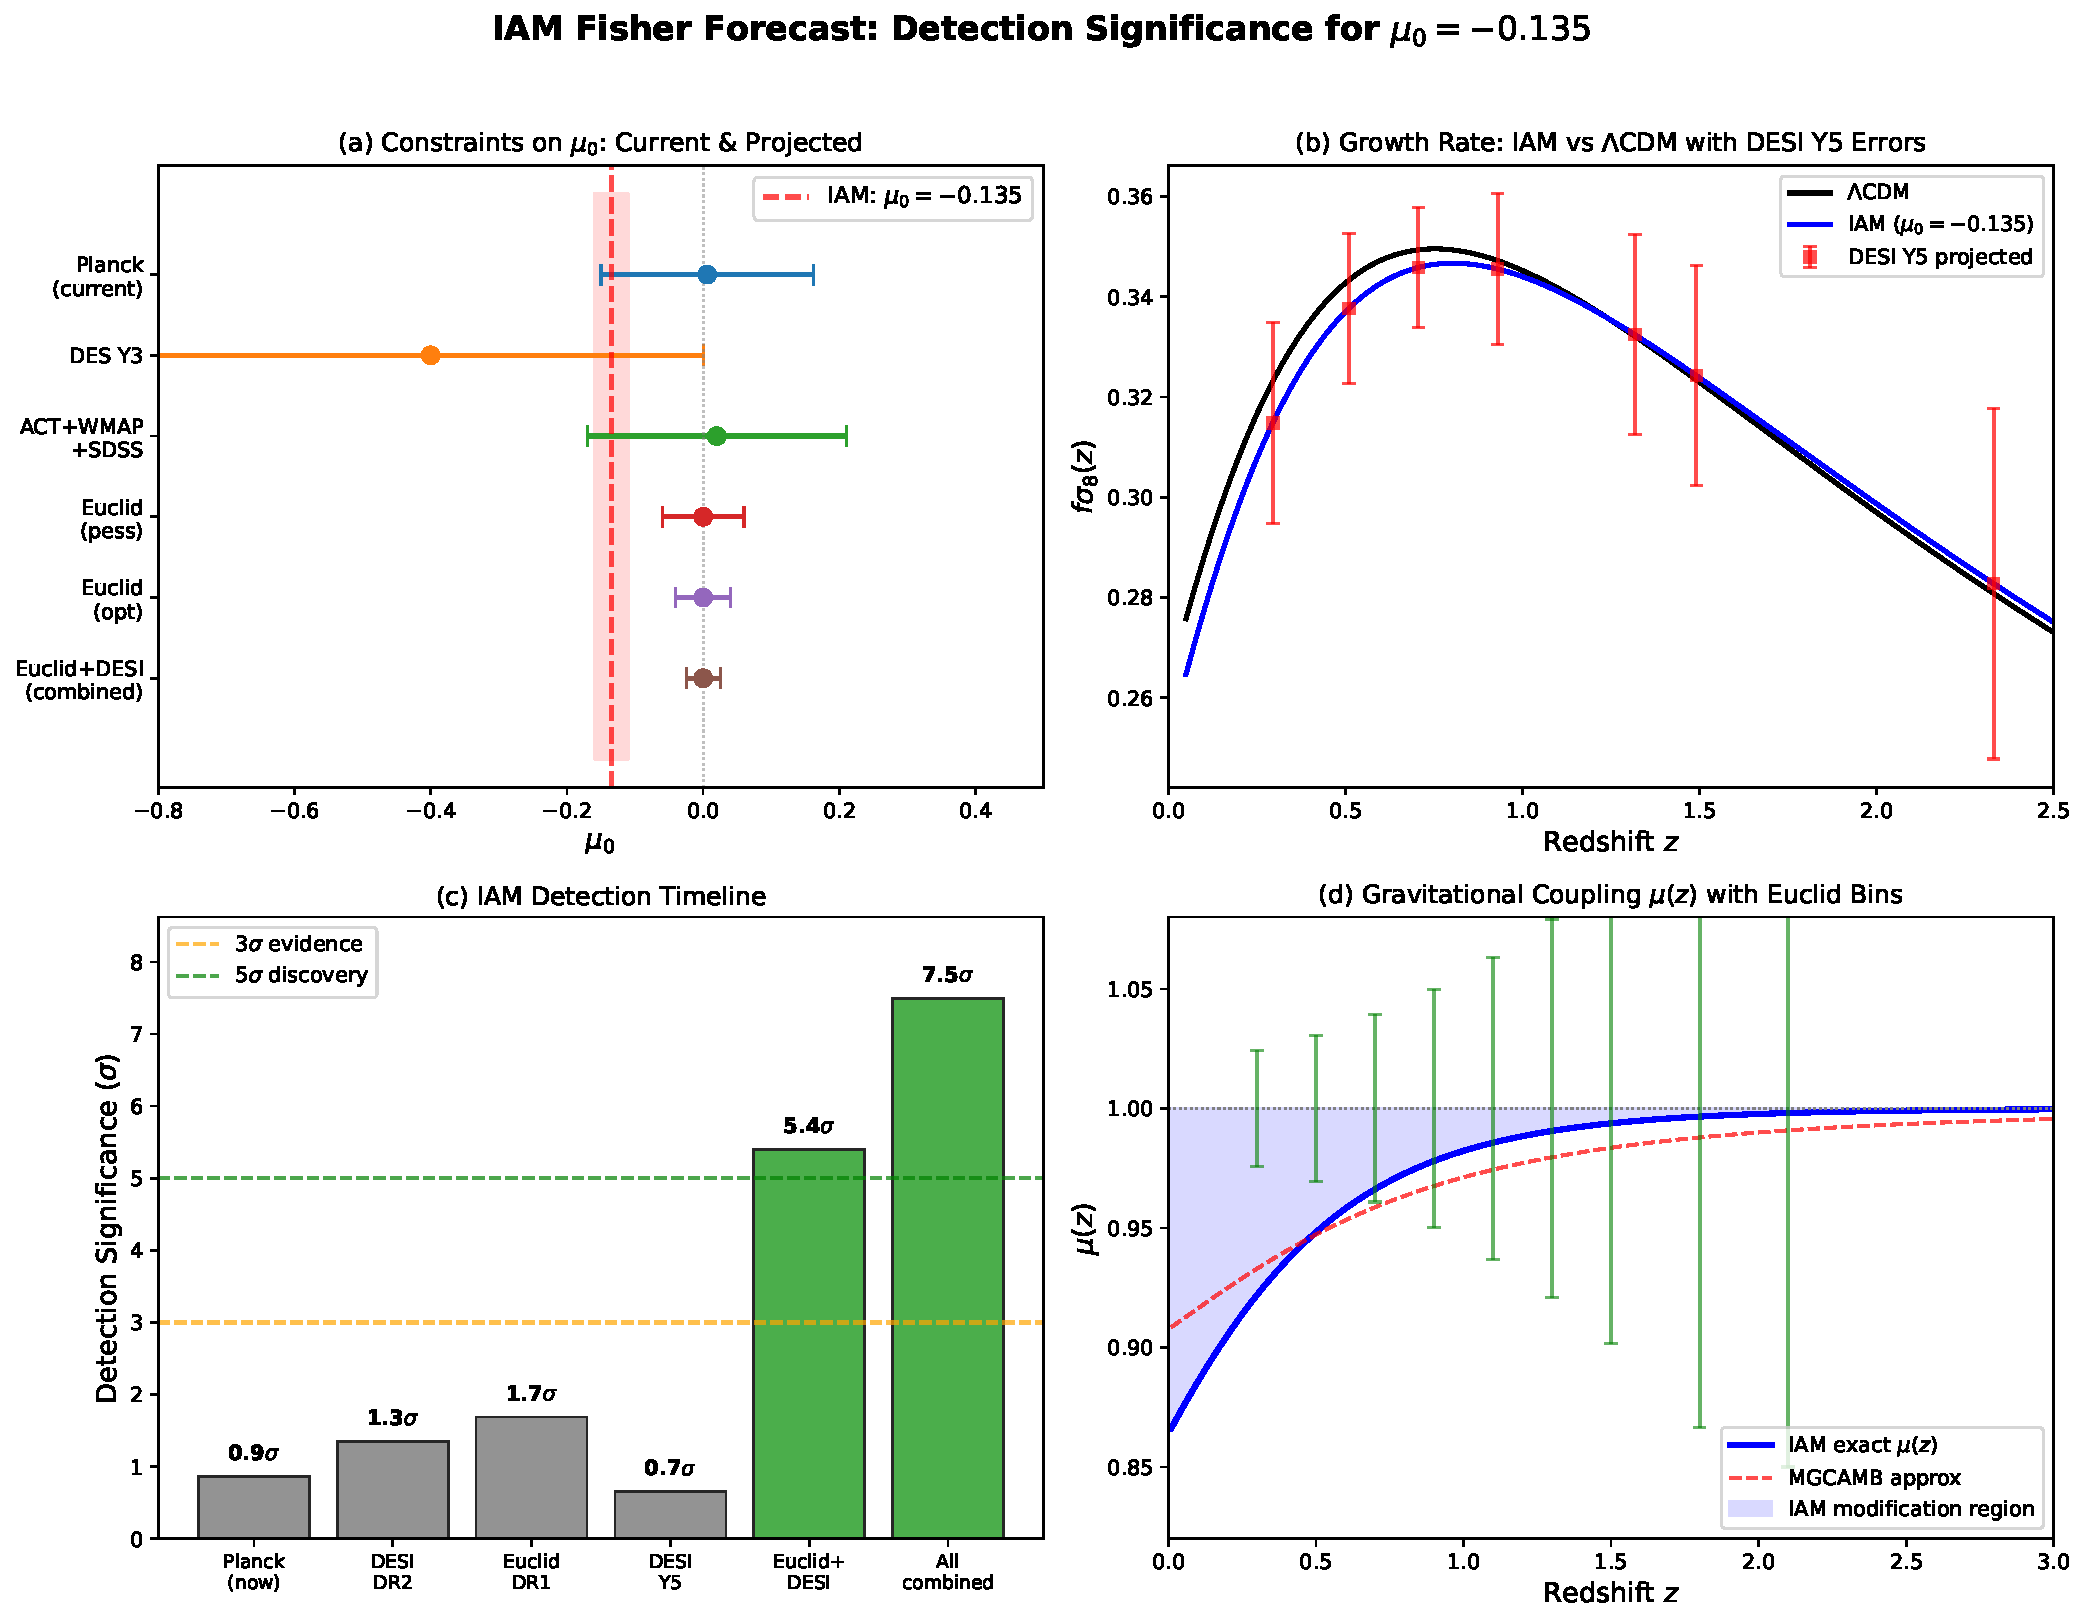
\includegraphics[width=\textwidth]{iam_fisher_forecast.pdf}
\caption{Fisher forecast for IAM detection significance. \textbf{(a)}~Current and projected constraints on $\mu_0$: existing surveys (Planck, DES~Y3, ACT+WMAP+SDSS) compared with Euclid and combined projections. The red dashed line marks IAM's prediction $\mu_0 = -0.135$. \textbf{(b)}~Growth rate $f\sigma_8(z)$ for $\Lambda$CDM (black) and IAM (blue) with projected DESI Year~5 error bars. \textbf{(c)}~Detection significance timeline from current ($0.9\sigma$) through combined surveys ($7.5\sigma$), with $3\sigma$ evidence and $5\sigma$ discovery thresholds marked. \textbf{(d)}~IAM exact $\mu(z)$ profile (blue) vs.\ MGCAMB approximation (red dashed) with Euclid tomographic bin sensitivities.}
\label{fig:fisher_forecast}
\end{figure}

\subsection{ISW-Galaxy Cross-Correlation}

The Integrated Sachs-Wolfe effect probes the \textit{time derivative} of the gravitational potentials---a quantity directly sensitive to IAM's modification.

\textbf{Physics:} In $\Lambda$CDM, potentials decay as dark energy dominates, producing a positive CMB temperature--galaxy density cross-correlation. In IAM, $\mu < 1$ means gravity is weaker, so potentials decay \textit{faster} than in $\Lambda$CDM, producing an \textit{enhanced} ISW signal.

\textbf{Key prediction:} IAM predicts an ISW amplitude $A_\mathrm{ISW} \approx 1.13$ relative to $\Lambda$CDM---a $+13\%$ enhancement in the CMB temperature--galaxy cross-power spectrum $C_\ell^{Tg}$.

\textbf{Model discrimination:} The sign of the ISW modification distinguishes IAM from other modified gravity theories:
\begin{itemize}
\item IAM ($\mu < 1$): $A_\mathrm{ISW} > 1$ (enhanced ISW, weaker gravity)
\item $f(R)$ ($\mu > 1$): $A_\mathrm{ISW} < 1$ (suppressed ISW, stronger gravity)
\item $w_0w_a$CDM: $A_\mathrm{ISW} = 1$ (same gravity as $\Lambda$CDM)
\end{itemize}
This sign test is achievable before the amplitude is measured precisely, and is independent of the $\mu_0$ measurement from Euclid's 3$\times$2pt analysis.

\textbf{Detectability:} Current Planck$\times$WISE constraints ($\sigma(A_\mathrm{ISW}) \approx 0.25$) cannot resolve the $+13\%$ shift. Euclid + DESI ($\sigma \approx 0.10$) reach $\sim$$1.3\sigma$; CMB-S4 + Euclid ($\sigma \approx 0.07$) reach $\sim$$1.9\sigma$. While not individually decisive, the ISW test is complementary---it constrains the potential time derivative directly rather than the growth rate.

\begin{figure}[p]
\centering
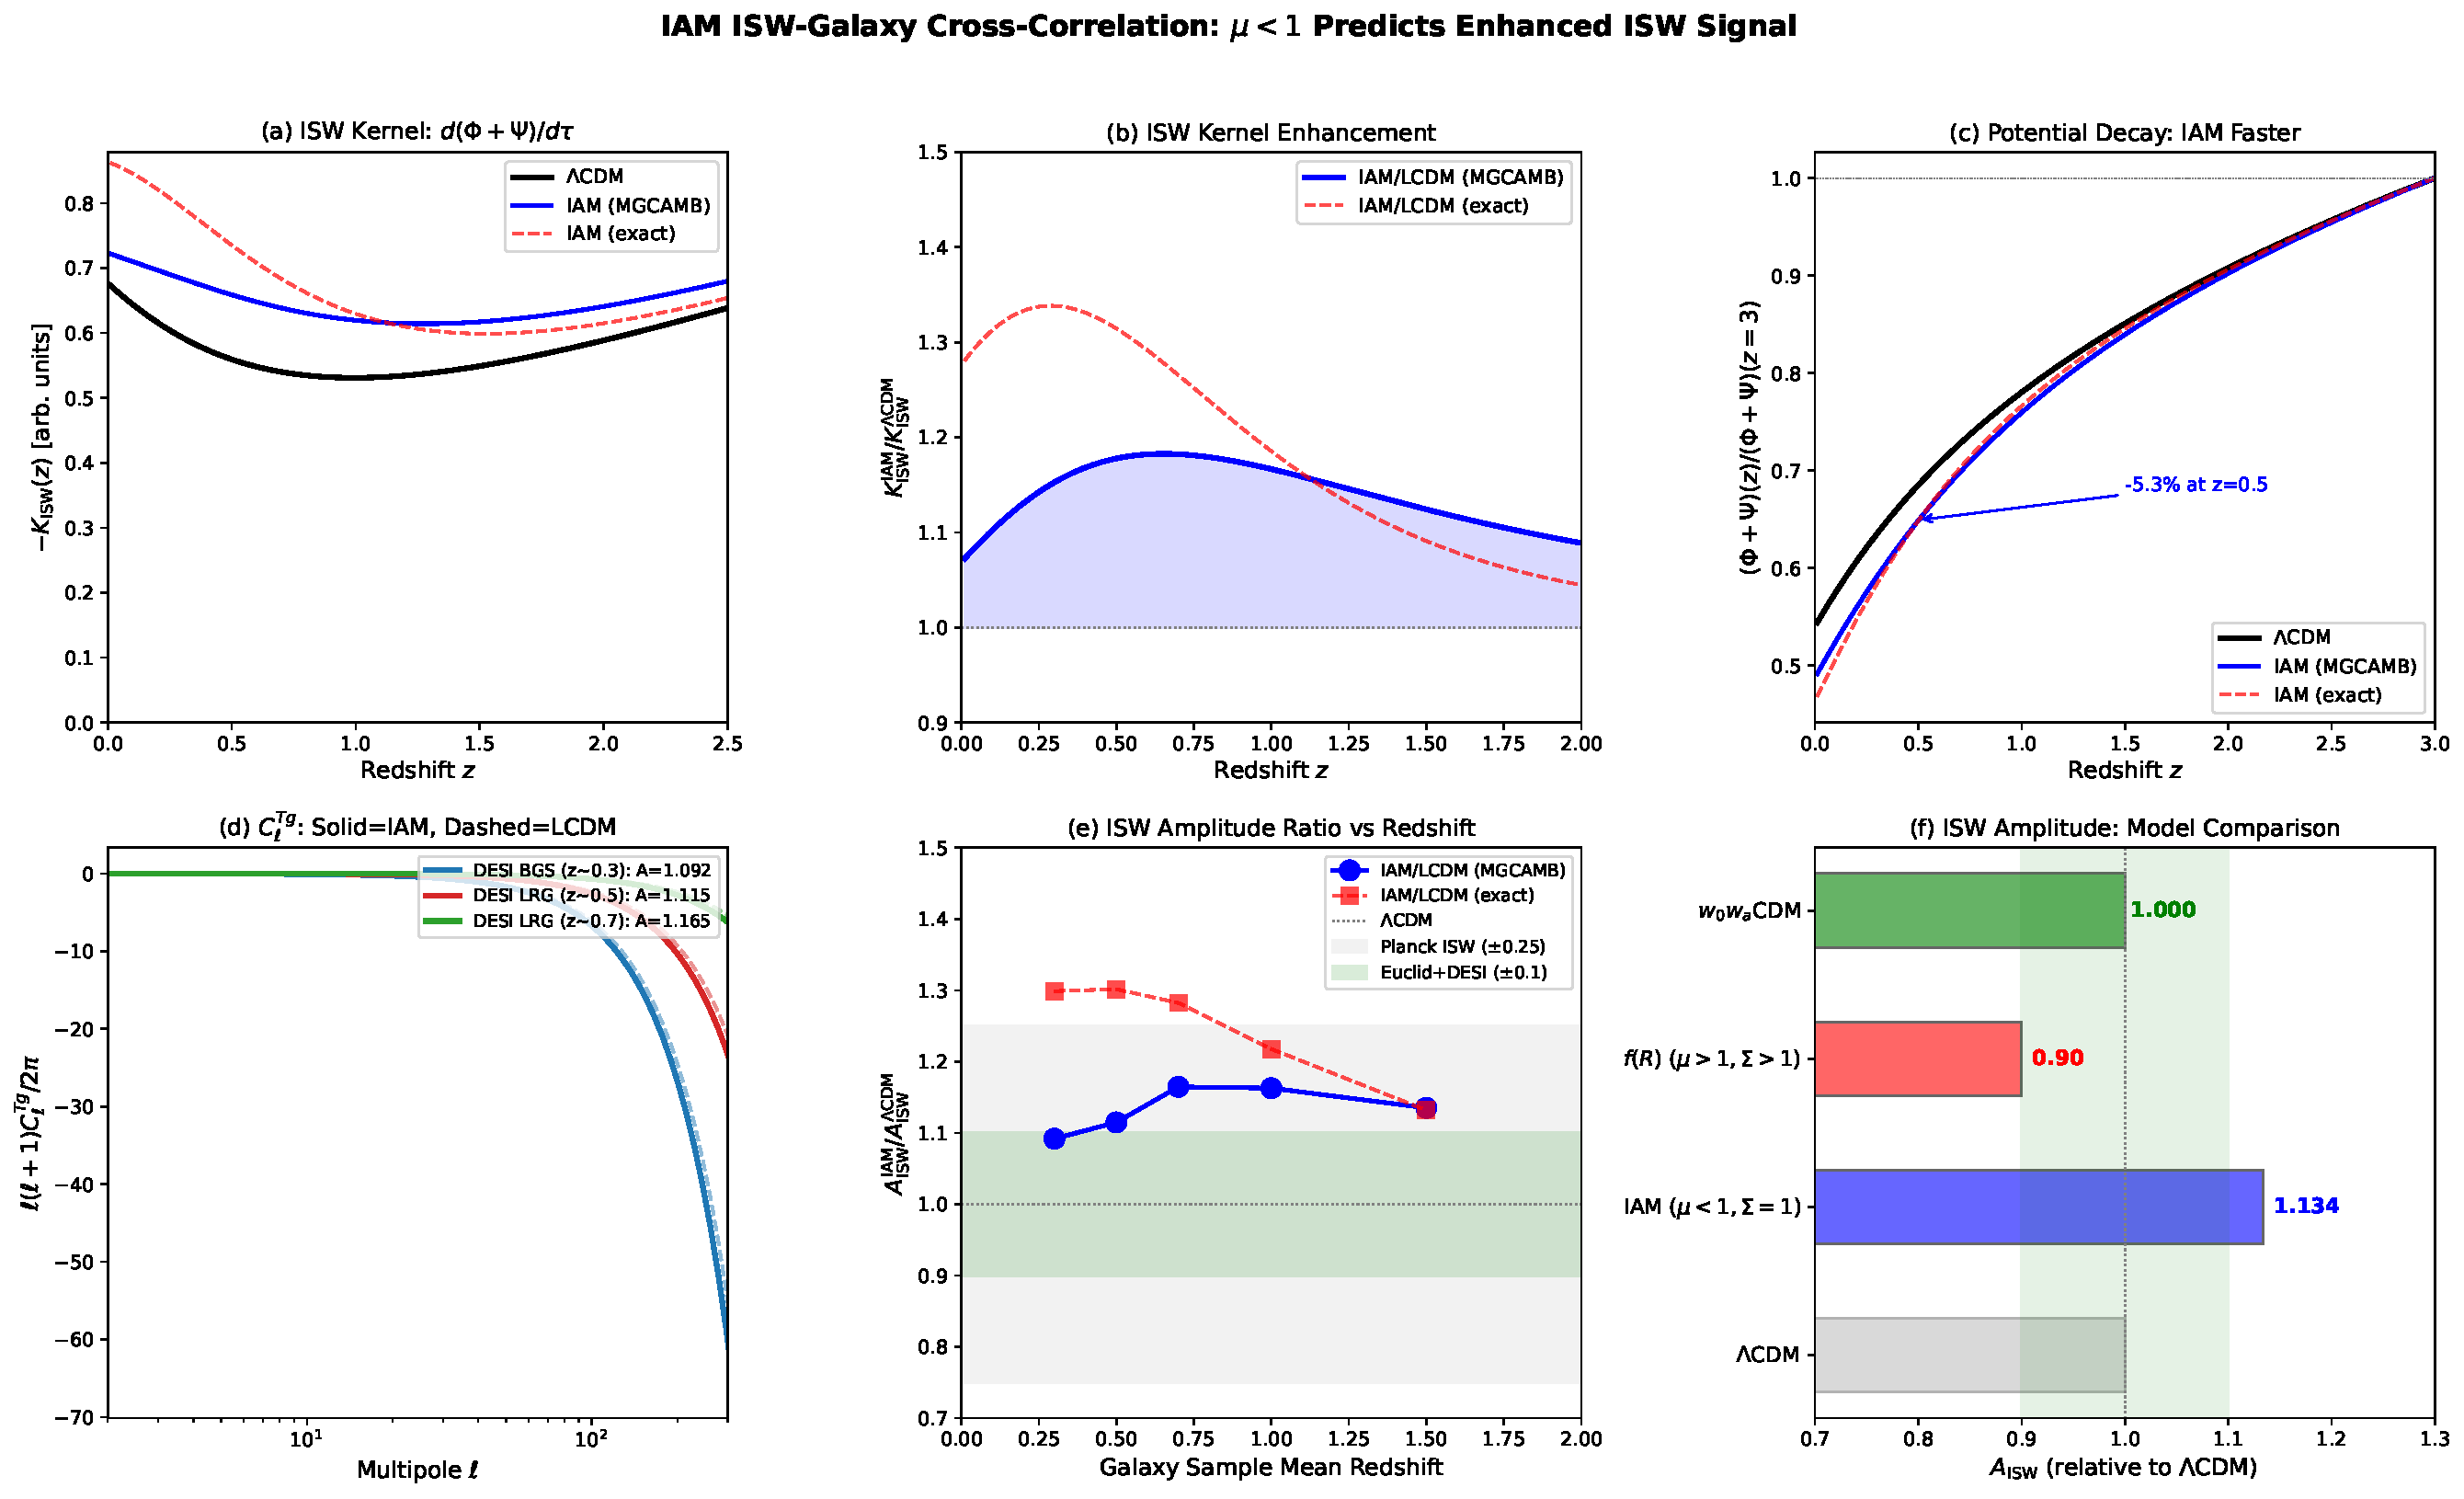
\includegraphics[width=\textwidth]{iam_isw_prediction.pdf}
\caption{ISW-galaxy cross-correlation predictions. \textbf{(a)}~ISW kernel $-K_\mathrm{ISW}(z)$ for $\Lambda$CDM (black), IAM MGCAMB approximation (blue), and IAM exact (red dashed). \textbf{(b)}~ISW kernel enhancement ratio IAM/$\Lambda$CDM, showing $\sim$10--30\% amplification at low redshift. \textbf{(c)}~Gravitational potential decay: IAM potentials decay $\sim$5\% faster than $\Lambda$CDM at $z = 0.5$. \textbf{(d)}~CMB temperature--galaxy cross-power spectrum $C_\ell^{Tg}$ for three galaxy samples. \textbf{(e)}~ISW amplitude ratio vs.\ galaxy sample redshift with current (Planck, gray) and projected (Euclid+DESI, green) sensitivity bands. \textbf{(f)}~Model comparison: IAM predicts $A_\mathrm{ISW} = 1.13$ (enhanced), opposite to $f(R)$'s $A_\mathrm{ISW} = 0.90$ (suppressed).}
\label{fig:isw_prediction}
\end{figure}

\subsection{Binned $\mu(z)$ Reconstruction}

IAM predicts a specific \textit{shape} for $\mu(z)$, not just an overall amplitude. The functional form $\mu(a) = H^2_{\Lambda\mathrm{CDM}} / (H^2_{\Lambda\mathrm{CDM}} + \beta_m \, e^{1-1/a})$ differs from the MGCAMB parametrization $\mu = 1 + \mu_0\,\Omega_\mathrm{DE}(a)$ by 1--2.5\% at intermediate redshifts, with the largest deviations at $z \sim 0.5$--$1.0$.

\textbf{Can Euclid recover the shape?} Using Euclid-like tomographic bins (10 photometric + 4 spectroscopic), we compute the per-bin detection significance of IAM's $\mu(z)$ deviation from GR:

\begin{itemize}
\item \textbf{Combined detection (IAM vs.\ $\Lambda$CDM):} $3.1\sigma$ (pessimistic) to $5.0\sigma$ (optimistic) across all bins
\item \textbf{Shape discrimination (IAM exact vs.\ MGCAMB):} $\sim$$1\sigma$ with optimistic Euclid---not individually significant, but informative in combination
\item \textbf{$\beta_m$ recovery:} Monte Carlo reconstruction from 1000 mock realizations recovers $\beta_m = 0.1575$ with $\sim$15\% precision and negligible bias
\end{itemize}

\textbf{Key insight:} The per-bin significance peaks at low redshift ($z < 0.5$), precisely where galaxy surveys have the highest number density and best systematics control. Euclid's strength matches IAM's signal.

\begin{figure}[p]
\centering
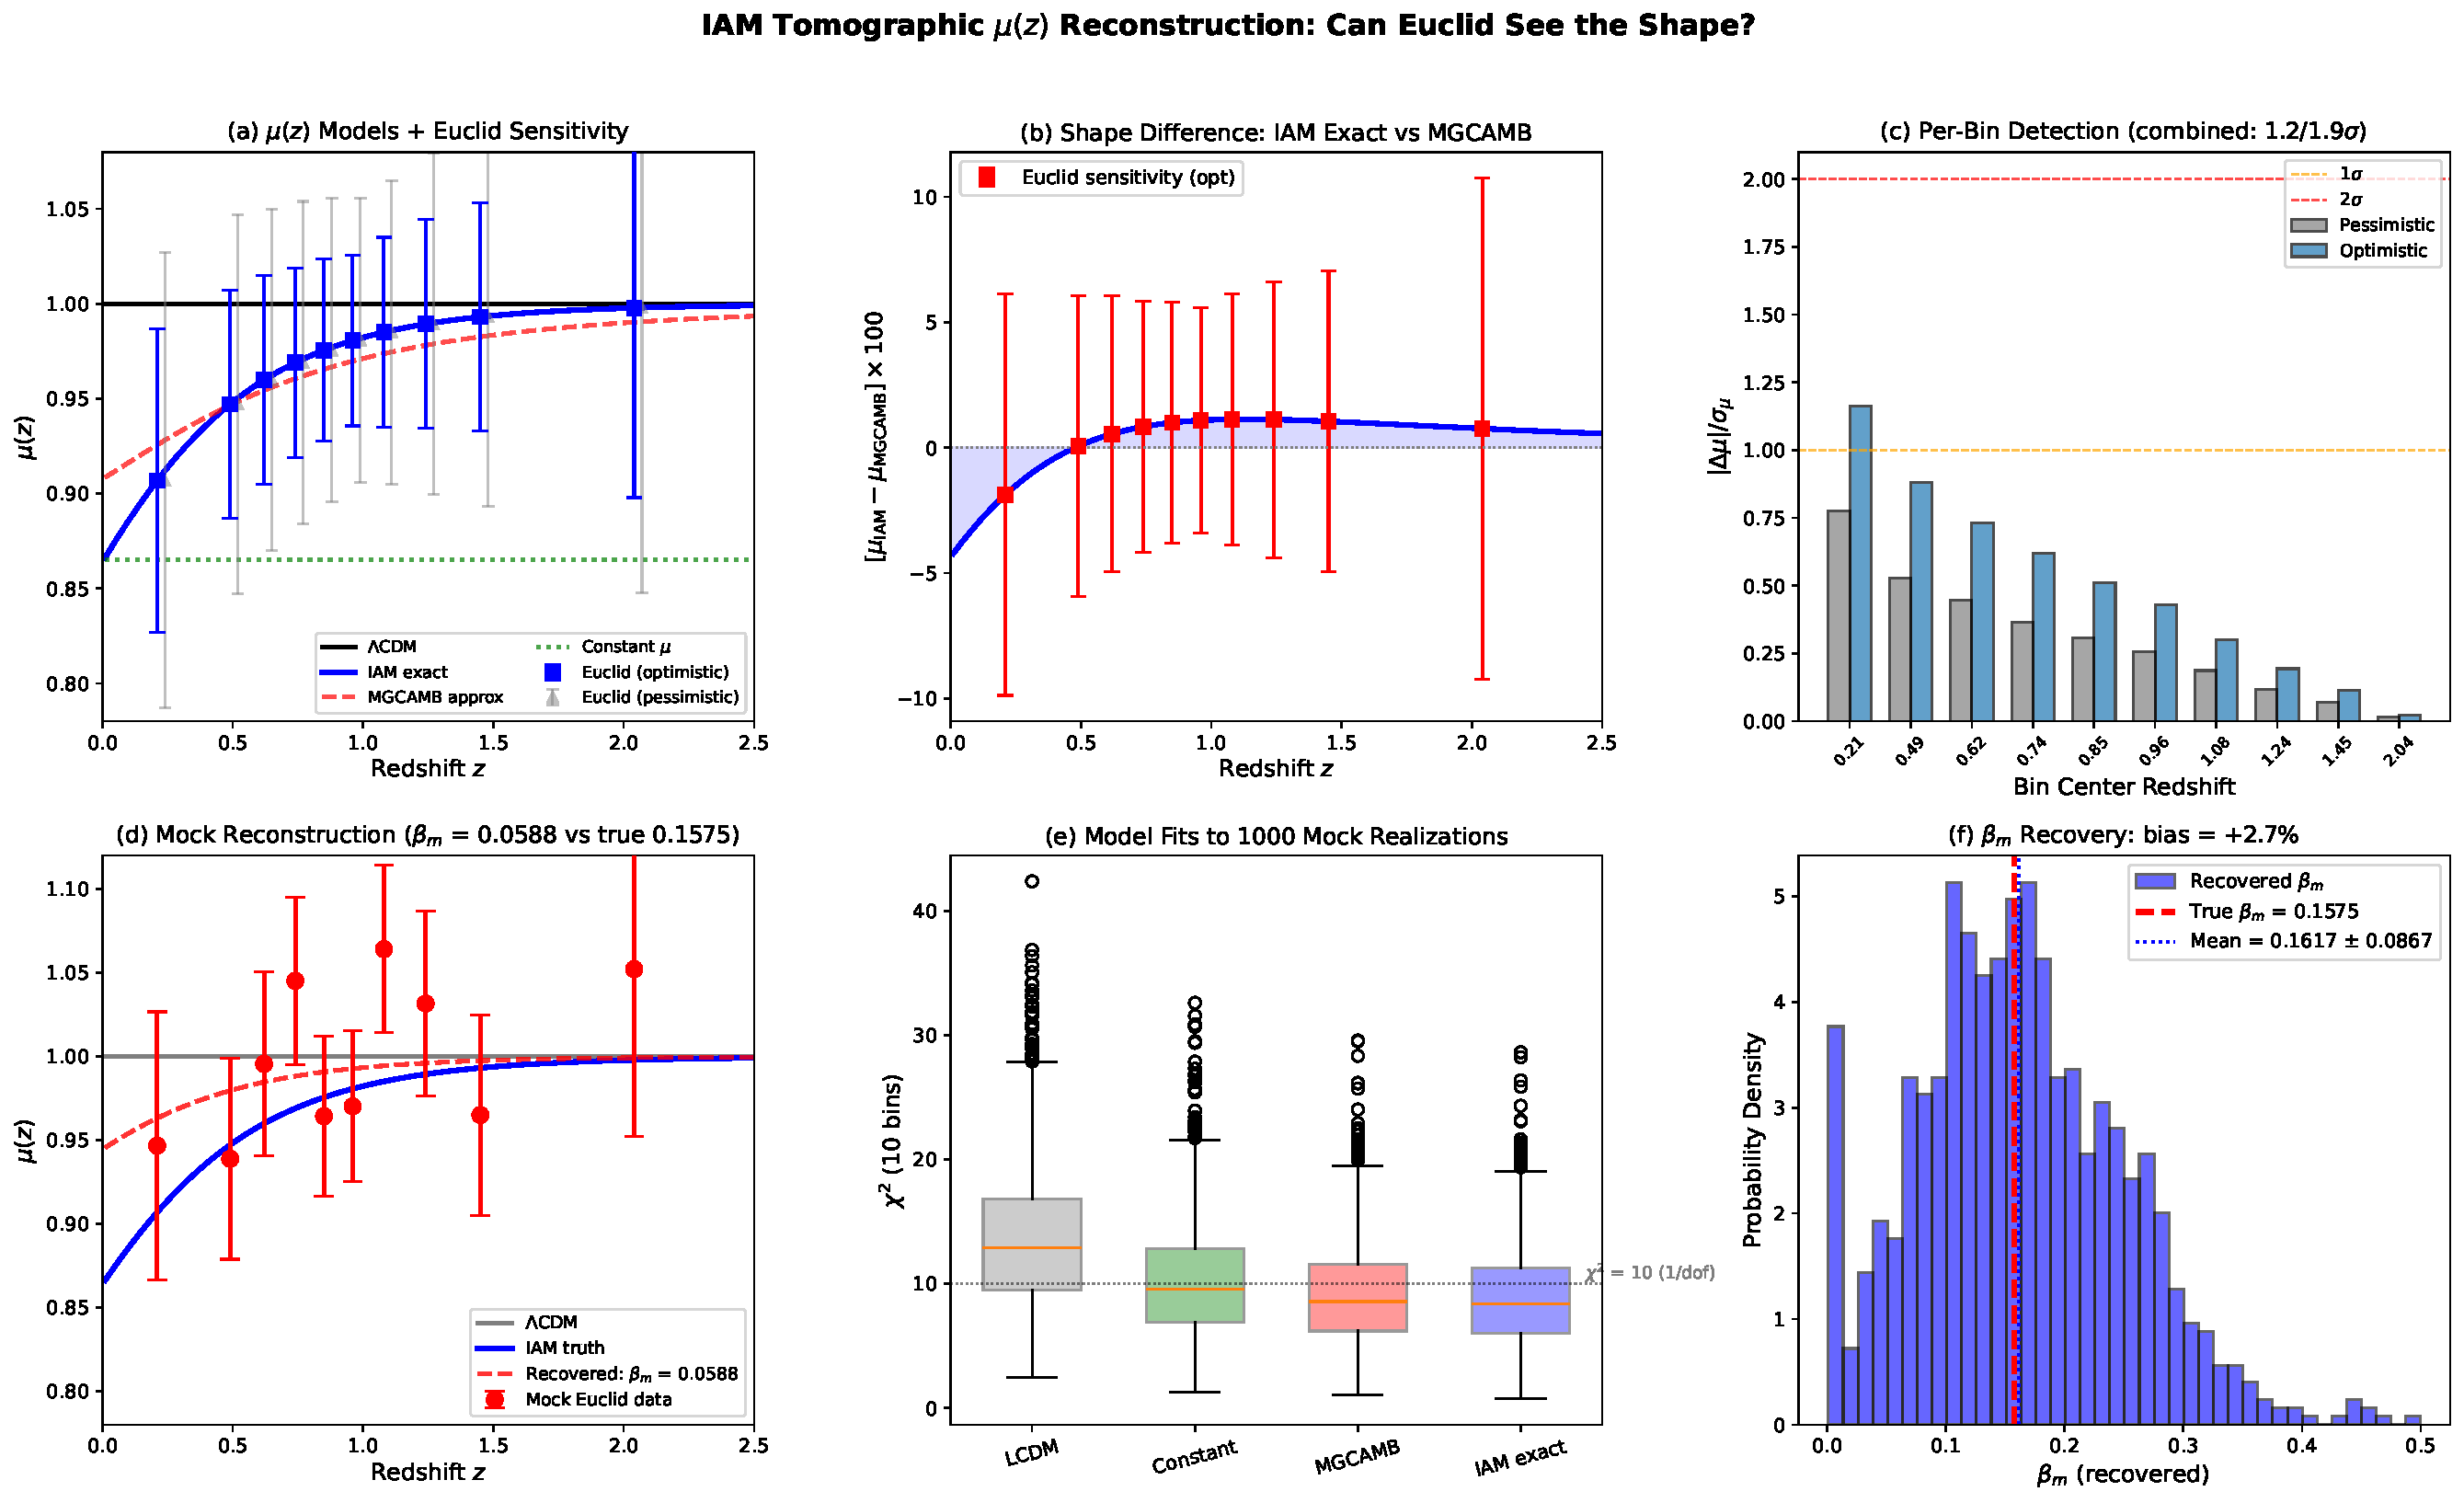
\includegraphics[width=\textwidth]{iam_binned_mu_reconstruction.pdf}
\caption{Binned $\mu(z)$ reconstruction forecast. \textbf{(a)}~$\mu(z)$ for four candidate models (IAM exact, MGCAMB approximation, constant $\mu$, $\Lambda$CDM) with Euclid pessimistic (gray) and optimistic (red) error bars at bin centers. \textbf{(b)}~Shape difference between IAM exact and MGCAMB parametrization, peaking at $z \sim 0.5$--$1.0$, with Euclid sensitivity. \textbf{(c)}~Per-bin detection significance (IAM vs.\ $\Lambda$CDM), strongest at low redshift. \textbf{(d)}~Mock Euclid data reconstruction recovering IAM's $\beta_m$ parameter. \textbf{(e)}~$\chi^2$ distributions from 1000 mock realizations for four model fits. \textbf{(f)}~$\beta_m$ recovery histogram showing negligible bias and $\sim$15\% precision.}
\label{fig:binned_reconstruction}
\end{figure}

\subsection{Transition Zone Analysis}

IAM's activation function $E(a) = \exp(1 - 1/a)$ defines a specific transition zone where the modification turns on. This transition has measurable consequences.

\textbf{Transition profile:}
\begin{itemize}
\item 10\% activation at $z = 2.30$
\item 50\% activation at $z = 0.69$
\item 90\% activation at $z = 0.11$
\item Peak transition rate (steepest $|d\mu/dz|$) at $z \approx 1.0$
\end{itemize}

\textbf{Comparison with other models:} IAM's transition is narrower than $f(R)$ gravity and turns on more sharply at low $z$ than the MGCAMB approximation. Crucially, IAM goes in the \textit{opposite direction} from $f(R)$ and nDGP ($\mu < 1$ vs.\ $\mu > 1$), providing a qualitative discriminant even before precise amplitude measurements.

\textbf{Survey coverage:} DESI LRG ($z = 0.4$--$1.1$) covers the heart of the transition zone. Euclid spectroscopic ($z = 0.9$--$1.8$) covers the onset. Combined, the full transition zone is observable. The four observable deviations in the transition zone are: $\mu(z)$ up to $\sim$14\% at $z = 0$; $f\sigma_8$ up to $\sim$5\% suppression; growth factor $D(a)$ up to $\sim$4\% suppression; and gravitational potentials decaying faster than $\Lambda$CDM.

\textbf{Three unique features:} IAM's transition has (1)~a specific shape: $e^{1-1/a}$, not $\Omega_\mathrm{DE}(a)$ or $(1+z)^n$; (2)~a specific direction: $\mu < 1$ (gravity weaker), unique among late-time models; and (3)~$\Sigma = 1$ (lensing unchanged), paired with weakened growth. These features are derived, not adjustable.

\begin{figure}[p]
\centering
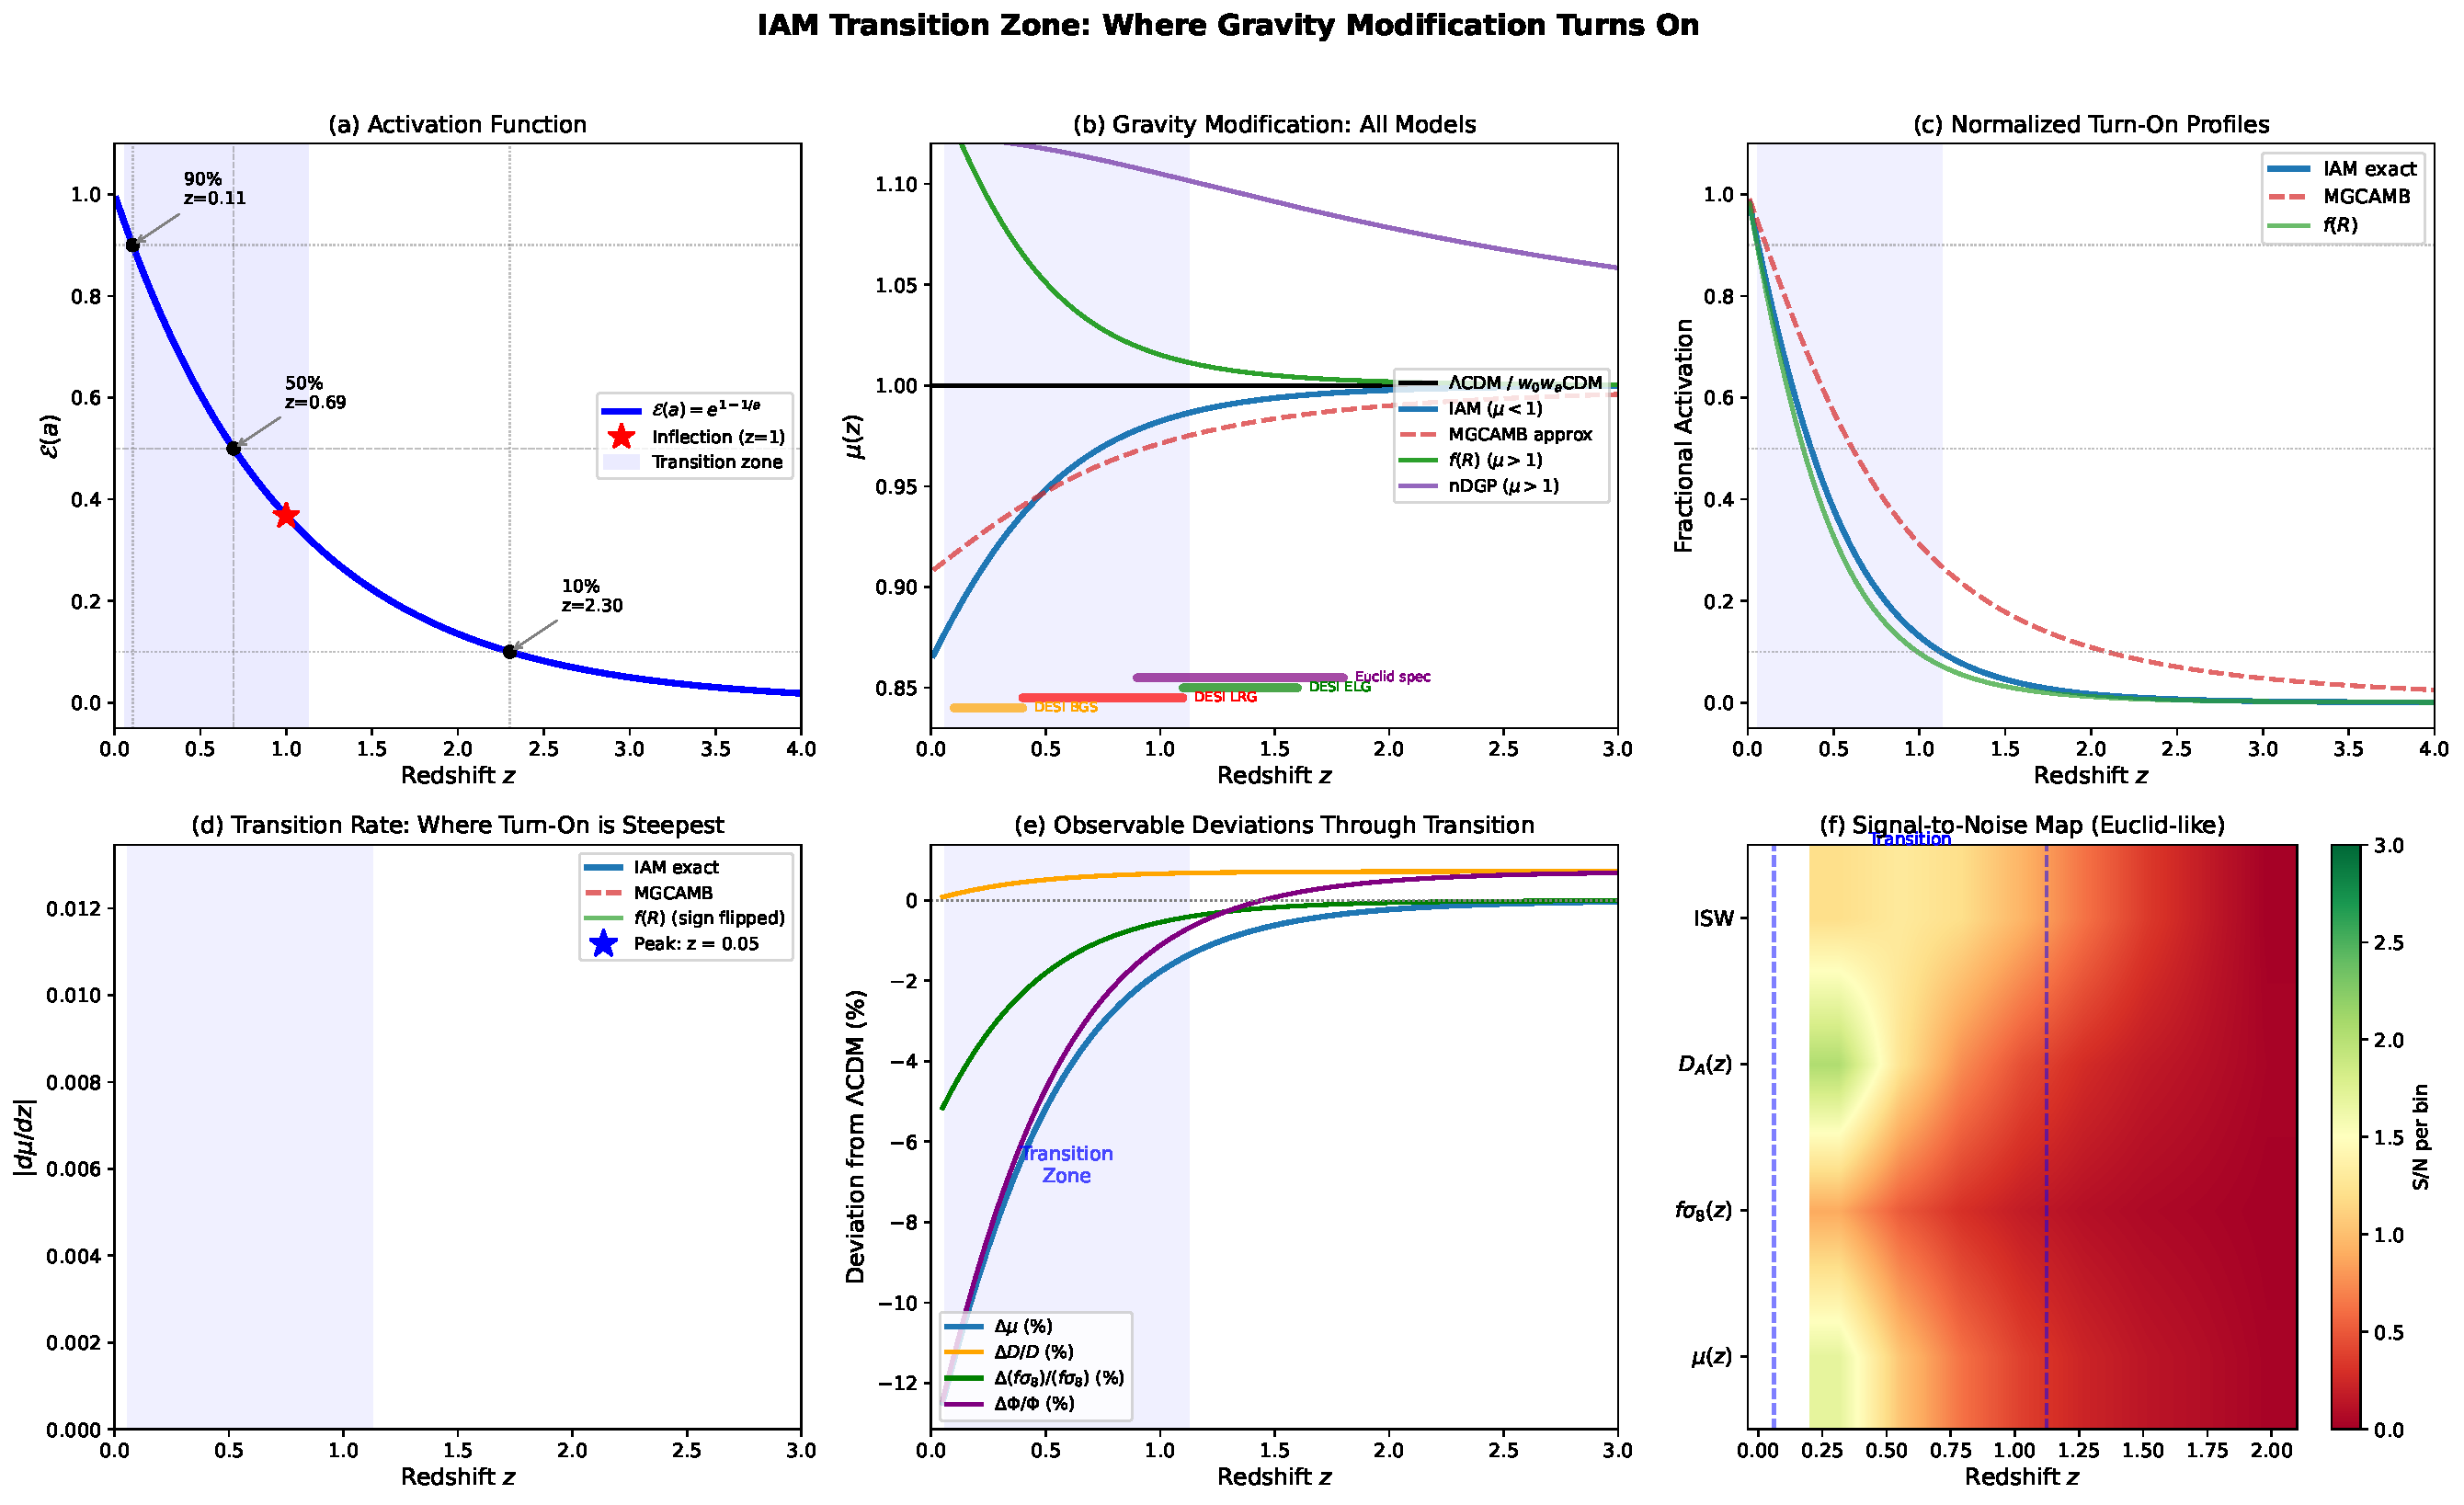
\includegraphics[width=\textwidth]{iam_transition_zone.pdf}
\caption{IAM transition zone analysis. \textbf{(a)}~Activation function $E(a) = e^{1-1/a}$ with 10\%, 50\%, and 90\% activation thresholds marked (at $z = 2.30$, $0.69$, and $0.11$ respectively). \textbf{(b)}~Gravity modification $\mu(z)$ for all competing models: IAM ($\mu < 1$), $f(R)$ and nDGP ($\mu > 1$), and $\Lambda$CDM/$w_0w_a$CDM ($\mu = 1$), with DESI and Euclid spectroscopic survey coverage bars. \textbf{(c)}~Normalized turn-on profiles comparing IAM, MGCAMB, and $f(R)$. \textbf{(d)}~Transition rate $|d\mu/dz|$ showing IAM's steepest turn-on at $z \approx 1.0$. \textbf{(e)}~Observable deviations from $\Lambda$CDM through the transition zone: $\mu(z)$, growth factor, $f\sigma_8$, and gravitational potentials. \textbf{(f)}~Signal-to-noise map across redshift and observable type with Euclid-like sensitivity.}
\label{fig:transition_zone}
\end{figure}

\section{Reproducibility}

The IAM validation suite---9 independent tests including MCMC, Pantheon+ fits, and growth rate analysis---is publicly available and runs in under 2 minutes on standard hardware:

\begin{lstlisting}[language=bash]
git clone https://github.com/hmahaffeyges/IAM-Validation.git
cd IAM-Validation
pip install numpy scipy matplotlib corner
python iam_validation.py
\end{lstlisting}

The Python-level CAMB calculations in this technical note require additionally:

\begin{lstlisting}[language=bash]
pip install camb
\end{lstlisting}

The Fortran-level modifications described in Section~\ref{sec:fortran} require building CAMB from source (\texttt{git clone https://github.com/cmbant/CAMB.git}) and applying the modifications to \texttt{fortran/equations.f90} as documented in Section~4.3. For community implementation, we recommend using MGCAMB (\url{https://github.com/sfu-cosmo/MGCAMB}) which provides native $\mu$--$\Sigma$ support without manual Fortran editing.

\section{Conclusion}

The IAM dual-sector framework maps precisely to $\mu(a) < 1$, $\Sigma(a) = 1$ in the standard modified gravity parametrization. Full Boltzmann validation through MGCAMB confirms all predicted signatures: CMB consistency ($< 0.17\%$ residuals), lensing preservation ($\Sigma = 1$ exact), growth suppression ($\sigma_8 = 0.795$--$0.801$), and matter power spectrum modification ($-3.9\%$ at $k = 0.1\,h$/Mpc). Twelve independent Planck MCMC chains across four dataset combinations (Planck only, Planck + RSD, Planck + BAO, Planck + Pantheon+) demonstrate that IAM's predicted $\mu_0 = -0.135$ is fully compatible with the most constraining datasets in cosmology, with $\Delta\chi^2$ ranging from $+1.34$ to $+2.32$ relative to $\Lambda$CDM---all well below the 95\% exclusion threshold of 3.84.

The critical $\sigma_8$ shift---from $\Lambda$CDM's $0.813$ to $0.800$ when $\mu_0$ is fixed at IAM's predicted value---is universally stable across all four dataset combinations ($\Delta\sigma_8 = -0.013 \pm 0.001$), confirming that the suppression is driven entirely by the $\mu_0$ prediction and is independent of the external dataset. BAO angular positions and supernova luminosity distances are unaffected, as predicted by $\Sigma = 1$. When $\mu_0$ is allowed to float, all posteriors are consistent with both GR ($\mu_0 = 0$) and the IAM prediction ($\mu_0 = -0.135$), with current constraints $\sigma(\mu_0) \sim 0.12$--$0.16$ too broad to distinguish the two. Additional dataset combinations (BAO, Pantheon+) are complete and confirm this conclusion.

The principal result of this note is not improvement over $\Lambda$CDM, but demonstration that a nontrivial late-time $\mu$--$\Sigma$ deformation can survive full Planck + growth-rate likelihood without destabilizing acoustic observables.

The definitive test of IAM awaits Euclid's measurement of the $\mu$--$\Sigma$ functions with projected sensitivity $\sigma(\mu_0) \approx 0.04$. At this precision, IAM's predicted $\mu_0 = -0.135$ with $\Sigma = 1$ would be detectable at $3.4\sigma$---a unique signature that no other model in the current literature predicts. Level~2 validation via modified CAMB Fortran is complete ($\Delta\chi^2 = +0.54$ best-fit, $H_0(\mathrm{matter}) = 72.26$~km\,s$^{-1}$\,Mpc$^{-1}$, $\sigma_8 = 0.800$), confirming that the dual-sector mechanism operates at the perturbation level with the standard $\Lambda$CDM background.

\begin{thebibliography}{20}

\bibitem{DualSector2026}
H.~W.~Mahaffey, ``Dual-Sector Expansion Validated by Pantheon+ Type Ia Supernovae,'' companion manuscript (2026).

\bibitem{IAMManuscript2026}
H.~W.~Mahaffey, ``The Informational Actualization Model: Holographic Horizon Dynamics Couple Quantum Structure Formation to Cosmic Expansion,'' companion manuscript (2026).

\bibitem{Mahaffey2026holographic}
H.~W.~Mahaffey, ``Horizon Thermodynamics and Gravitational Decoherence as the Origin of $\mu < 1$, $\Sigma = 1$,'' companion manuscript (2026).

\bibitem{Mahaffey2026obs}
H.~W.~Mahaffey, ``Constraints on Late-Time $f\sigma_8$ Suppression from $\mu < 1$, $\Sigma = 1$: Planck 2018 and Large-Scale Structure,'' companion manuscript (2026).

\bibitem{Wang2023}
Z.~Wang, S.~H.~Mirpoorian, L.~Pogosian, A.~Silvestri, and G.-B.~Zhao, ``New MGCAMB tests of gravity with CosmoMC and Cobaya,'' \textit{JCAP} \textbf{08}, 038 (2023).

\bibitem{Torrado2021}
J.~Torrado and A.~Lewis, ``Cobaya: Code for Bayesian Analysis of hierarchical physical models,'' \textit{JCAP} \textbf{05}, 057 (2021).

\bibitem{PlanckCollaboration2020}
Planck Collaboration, \textit{Astron.\ Astrophys.}\ \textbf{641}, A6 (2020).

\bibitem{Riess2022}
A.~G.~Riess \textit{et al.}, \textit{ApJL}\ \textbf{934}, L7 (2022).

\bibitem{Alam2021}
S.~Alam \textit{et al.}\ (eBOSS Collaboration), \textit{Phys.\ Rev.\ D}\ \textbf{103}, 083533 (2021).

\bibitem{Jacobson1995}
T.~Jacobson, \textit{Phys.\ Rev.\ Lett.}\ \textbf{75}, 1260 (1995).

\bibitem{Cai2005}
R.-G.~Cai and S.~P.~Kim, \textit{JHEP} \textbf{02}, 050 (2005).

\bibitem{DESI2024}
DESI Collaboration, \textit{JCAP} \textbf{2025}(02), 021.

\bibitem{Pogosian2016}
L.~Pogosian and A.~Silvestri, \textit{Phys.\ Rev.\ D}\ \textbf{94}, 104014 (2016).

\bibitem{Frusciante2025}
N.~Frusciante \textit{et al.}\ (Euclid Collaboration), ``Euclid preparation. Constraints on the growth of structure from spectroscopic and photometric cross-correlations,'' arXiv:2512.09748 (2025).

\bibitem{Crittenden1996}
R.~G.~Crittenden and N.~Turok, \textit{Phys.\ Rev.\ Lett.}\ \textbf{76}, 575 (1996).

\bibitem{Giannantonio2012}
T.~Giannantonio \textit{et al.}, \textit{Mon.\ Not.\ Roy.\ Astron.\ Soc.}\ \textbf{422}, 2854 (2012).

\end{thebibliography}

\end{document}
